\chapter{Analysis}
This chapter contains an extensive discussion of the data analysis techniques in the physics measurement. First we describe the building blocks of the  $v_2$ measurement, then we examine the event plane analysis techniques and the sources of systematic uncertainty.
\section{The Building Blocks of the Measurement}
Prior to any analysis, the raw data collected by various PHENIX subsystems must be reconstructed into well-defined software objects encapsulating information of the particles that traversed the detector. Although we have already discussed the subsystems used in this analysis in Chapter 3, this section provides in-depth information on central arm tracks, FVTX clusters, and BBC photomultiplier tubes (PMTs), and the physics variables they contain. Figure \ref{fig:phenix_coord_system} displays the coordinate system for PHENIX and the particle parameters that are in relation to it.

%In this section, I will be detailing the relevant direct observables used in this measurement. They include parameters from central arm tracks, FVTX clusters, and BBC PMTs. Although the Central Arms, FVTX, and BBC have already been described in chapter 3, I will go into more detail into the parameters available and their mathematical precision. 

\begin{figure}[!ht]
\begin{center}
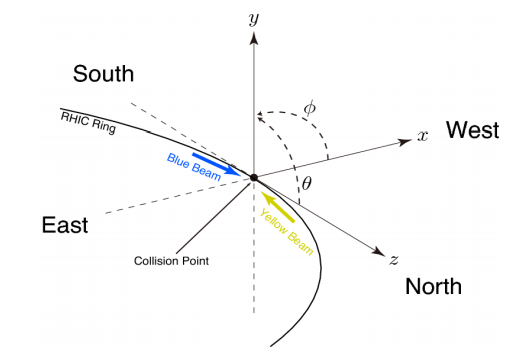
\includegraphics[width=0.55\linewidth]{figs/phenix_coord.png}
\caption{Reference coordinate system for the PHENIX detector. The origin is set at the collision point, around which the detector is centered. The beam runs parallel to the (longitudinal) $z-$axis, where the direction of positive $z$ is defined as \emph{north}. The \emph{east} and \emph{west} directions are defined as perpendicular to the longitudinal direction, where the direction of positive $x$ is defined as west.}
\label{fig:phenix_coord_system}
\end{center}
\end{figure}

%\begin{figure}[!h]
%\begin{center}
%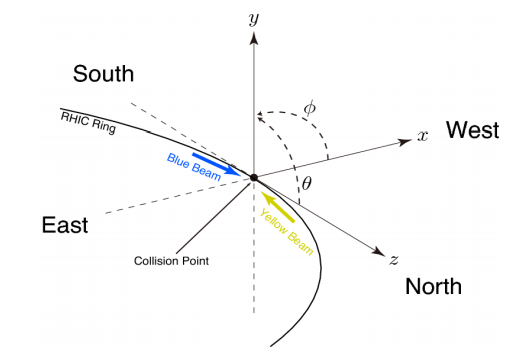
\includegraphics[width=0.55\linewidth]{figs/phenix_coord.png}
%\caption{For reference, I show the PHENIX coordinate system here. The origin is in the middle of the PHENIX detector at the collision %point. North and south are parallel to beam axis. East and west are transverse to the beam axis. Central detectors have a west and an %east arm on either side of the beam. Forward detectors have a north and a south arm relative to the origin.}
%\end{center}
%\end{figure}
%-todo: list all parameters used in the analysis. show some performance plots
\subsection{Central Arm Tracks}
Central Arm (CA) tracks are the representation of charged particles emitted from the heavy ion collision, which are detected by detectors in the PHENIX central arms. There are two central arms, each one covering an acceptance of $\pm 0.35$ in pseudorapidity and a total azimuth acceptance of $\frac{\pi}{2}$. The relevant detectors in the CA for this analysis include the Drift Chamber (DC), the Pad Chambers (PC) and the Ring Imaging Cerenkov (RICH) detector. As discussed in Chapter 3, the DC provides momentum information; the PC provide track quality metrics; and the RICH provides electron identification. 

The main physical parameter of CA tracks is the momentum vector $\vec{p} = (p_x, p_y, p_z)$ of the particles, defined at the collision vertex. This analysis uses tracks with momentum 0.02 GeV/c $< |\pt| < 3.5$ GeV/c, a \pt range where the momentum resolution is good, as shown in the left panel of Figure \ref{fig:dc_mom_res}. The right panel of Figure \ref{fig:dc_mom_res} shows the \pt distribution of CA tracks up to 10 GeV/c: a smooth linearly falling distribution on a log scale with a small number of fake tracks at high \pt. The azimuthal angle and pseudorapidity of the track are calculated from the components of its momentum vector, as follows: 
\begin{align}
\phi &= \arctan( \frac{p_y}{p_x} ),\\
\eta &= \operatorname{arsinh}(\frac{p_z}{p_T}). 
\label{eqn:phi_eta_form}
\end{align}

\begin{figure}[!h]
\begin{center}
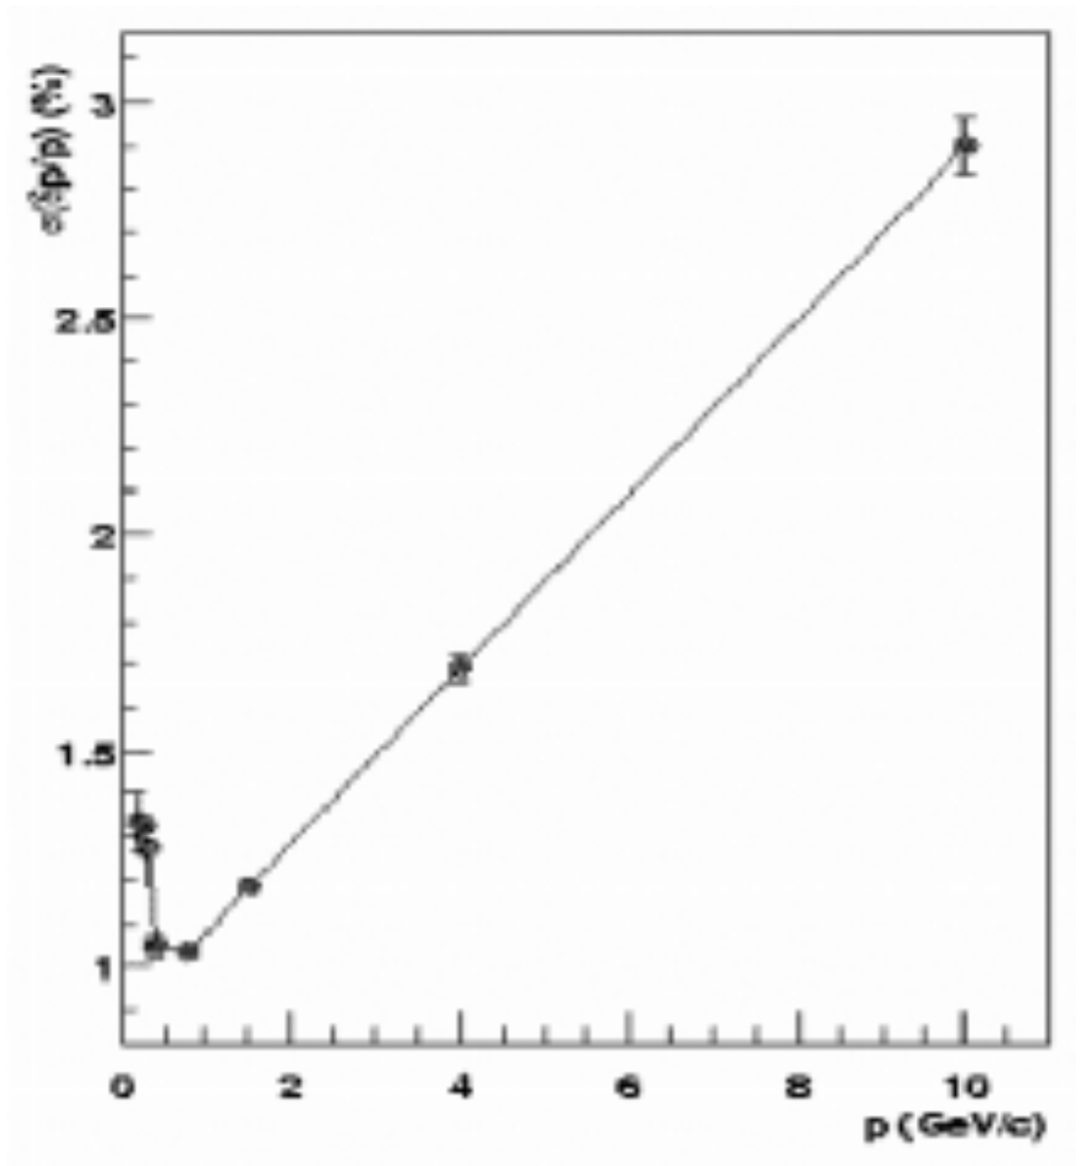
\includegraphics[width=0.4\linewidth]{figs/dc_mom_res.png}
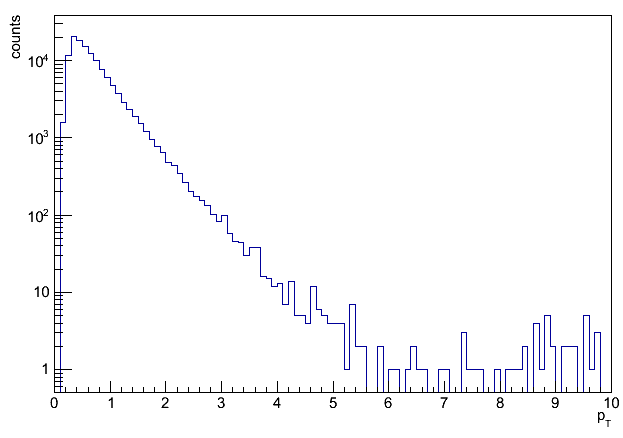
\includegraphics[width=0.45\linewidth]{figs/cnt_pt_dist.png}
\caption{Momentum resolution $\sigma_{p}/p$ as a function of the reconstructed track momentum, $p$ for simulated single-particle events~\cite{CA_spectro} (left) and the transverse momentum $p_{T}$ distribution of CA tracks in \pau events at \sqsn = 200 GeV. High $p_T$ tracks (\pt $>$ 5 GeV/c)observed correspond to unsubtracted background (right).}
\label{fig:dc_mom_res}
\end{center}
\end{figure}

\begin{figure}[!h]
\begin{center}
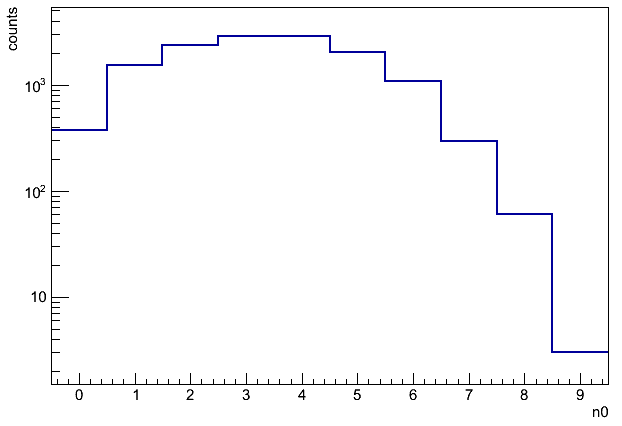
\includegraphics[width=0.45\linewidth]{figs/n0_dist.png}
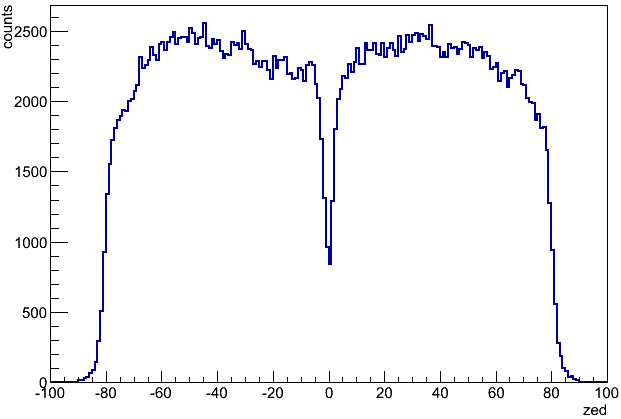
\includegraphics[width=0.45\linewidth]{figs/zed_dist.png}
\caption{The distribution of (left) $n0$, i.e., the number of PMTs fired in the RICH, and (right) $zed$, i.e., the longitudinal position of tracks in the DC, for CA tracks in 0--5\% central \pau events at \sqsn = 200 GeV. The structure observed in the $zed$ distribution corresponds to a gap in the detector acceptance.}
\label{fig:n0_and_zed}
\end{center}
\end{figure}

In addition to momentum, CA tracks provide a number of other parameters that can be used to ensure the quality of tracks and isolate a sample corresponding to charged hadrons. These include $zed$ in the DC, d$\phi$ and d$z$ in the PC, $n0$ in the RICH, and the general track quality calculated from DC and PC information. These variables are defined as follows:
\begin{itemize}
\item the $zed$ variable corresponds to the longitudinal position of the track in the DC, as shown in Fig. \ref{fig:n0_and_zed} (right panel);
\item the d$\phi$ and d$z$ variables quantify the distance between a track projection and its associated hits in the PC. In order to make standard cuts on these variables, their distribution must be calibrated to a standard Gaussian in a procedure known as sigmalization, described in subsection \ref{sec:pc_sigmala};
\item the $n0$ variable, used for electron identification, corresponds to the number of PMTs fired in the RICH that match the DC track projection, as shown in Fig. \ref{fig:n0_and_zed};
\item the track quality category, which is based on the PC1 and DC wire hits used as well as DC wire momentum information, defined in Tables \ref{tbl:dc_track_quality_pc1} and \ref{tbl:dc_track_quality_x1}.
\end{itemize}

\begin{table}[!ht]
\caption{Quality categorization of CA tracks, as a function of PC1 and DC wire hits. The quality parameters used in this analysis are 31 and 63 to maximize information available. Table from Ref~\cite{Belmont:2012pka}.}
\begin{center}
%    \begin{tabular}{| l | l | l | | | | | | }
    \begin{tabular}{ccccc}
    \hline
    Quality & PC1 found  & PC1 unique & UV found & UV unique\\ \hline
    17,18,19 & 1 & 0 & 0 & 0\\ \hline
    21,22,23 & 1 & 0 & 1 & 0\\ \hline
    29,30,31 & 1 & 0 & 1 & 1\\ \hline
    49,50,51 & 1 & 1 & 1 & 0\\ \hline
    61,62,63 & 1 & 1 & 1 & 1\\ \hline
    \end{tabular}
\end{center}
\label{tbl:dc_track_quality_pc1}
\end{table}

\begin{table}[!ht]
\caption{Quality categorization of CA tracks, as a function of DC wire momentum information. The quality parameters used in this analysis are 31 and 63 to maximize information available. Table from Ref~\cite{Belmont:2012pka}.}
\begin{center}
%    \begin{tabular}{| l | l | l | | | | | | }
    \begin{tabular}{ccc}
    \hline
    Quality & X1 used  & X2 used\\ \hline
    17,21,29,49,61 & 1 & 0 \\ \hline
    18,22,30,50,62 & 0 & 1 \\ \hline
    19,23,31,51,63 & 1 & 1 \\ \hline
    \end{tabular}
\end{center}
\label{tbl:dc_track_quality_x1}
\end{table}

The quality cuts Table \ref{tbl:cent_arm_trk_cut} summarizes the CA track cuts used in this analysis to reduce the track background. 
\begin{table}[!ht]
\caption{CA Track cuts for each relevant variable and their units.}
\begin{center}
    \begin{tabular}{| l | l | l | }
    \hline
    $variable$ & cuts  & units\\ \hline
    \pt & 0.02 $< p < $ 10.0  & GeV/c\\ \hline
    zed & $|zed| <$75  & cm \\ \hline
    PC3 d$\phi$ & $|d\phi|<$2.0  & radians $\times10^{9}$ \\ \hline
    PC3 dz & $|dz|<$2.0 & cm \\ \hline
    n0 & n0$<$1 & count \\ \hline
    quality & 63 or 31& N/A \\ \hline
    \end{tabular}
\end{center}
\label{tbl:cent_arm_trk_cut}
\end{table}

\subsubsection{Sigmalization of PC Variables}
\label{sec:pc_sigmala}
The goal of PC variables d$\phi$ and d$z$ is to provide criteria to determine if the $\phi$ orientation and $z$-direction of the track match between the third layer of the PC and the DC. The sigmalization is done in the minimum bias sample and is valid for all other centrality selections.
We did the sigmalization procedure for tracks in different transverse momentum bins, separately in the east
and west arms, and for positive and negative particles. The d$\phi$ and $d$z distributions
were fitted with a double-Gaussian function (one Gaussian for the signal and one Gaussian for the background) and then the parameters were interpolated as
a function of $p_T$. Fig. \ref{fig:pc3_sig} a) shows a fit to the sigmalized
d$\phi$ distribution, and Fig. \ref{fig:pc3_sig} b) shows a fit to the sigmalized d$z$ distribution for tracks with 1.0 $< p_T <$ 1.1 (GeV/c)
in both the west and east arms as well as both positively and negatively charged particles.
Then we fit the signal Gaussian mean and sigma to a polynomial function.  Once these variables had been sigmalized, we selected only
the tracks within a $\pm$2$\sigma$ cut.

\begin{figure}[!ht]
\begin{center}
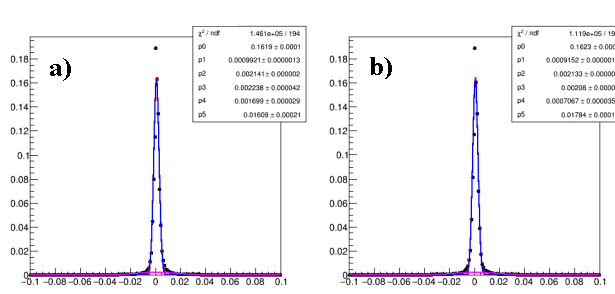
\includegraphics[scale=0.55]{figs/pc3dphi.png}
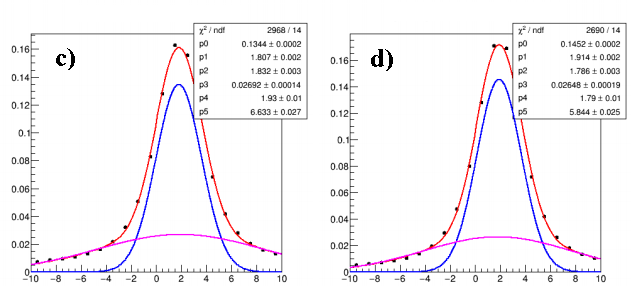
\includegraphics[scale=0.55]{figs/pc3dz.png}
\end{center}
\caption{The PC3 matching d$\phi$ fit in range 1.0 GeV/c $< \pt <$ 1.1 GeV/c for positive a) and negative b) hadrons and the d$z$ sigmalization for positive c) and negative d) hadrons. The blue and pink lines are single Gaussian fits to the signal and background, respectively, which are combined in the red line.
}
\label{fig:pc3_sig}
\end{figure}

%\subsection{Central Arm Tracking}

%In \pau collisions, the average number of reconstructed CNT (before cuts) is (\textbf{TO DO: QUANTIFY THIS}).
\subsection{FVTX Clusters}
The FVTX consists of four silicon layers in each of the north and south directions, covering an acceptance of $1 < | \eta | < 3$ and spanning the full azimuth. FVTX clusters correspond to the spatial location where charged particles hit one of the silicon layers. Each cluster is expected to correspond to a single charged particle in the case of \pau collisions, because of the low multiplicity relative to Au+Au collisions. These clusters have a spatial resolution in $r$ and $\phi$ of 50 $\mu$m and 0.14 radians, respectively, and have an RMS along the $z$-direction that corresponds to the width of an FVTX layer, of $\frac{200}{\sqrt{12}}$ $\mu$m \cite{Aidala201444}. Due to the \pau collision system's inherent asymmetry, the majority of particles are produced in Au-going (south or backward) direction. Taking into account this asymmetry, only the clusters from the south arm are used for calculations in this analysis. In a typical 0--5$\%$ centrality event, there are on average $\sim$1500 FVTX clusters in the south arm alone. Average hit distributions are shown in Figure \ref{fig:fvtx_clusxy}.

%%check numbers in this section
\begin{figure}[!ht]
\centering
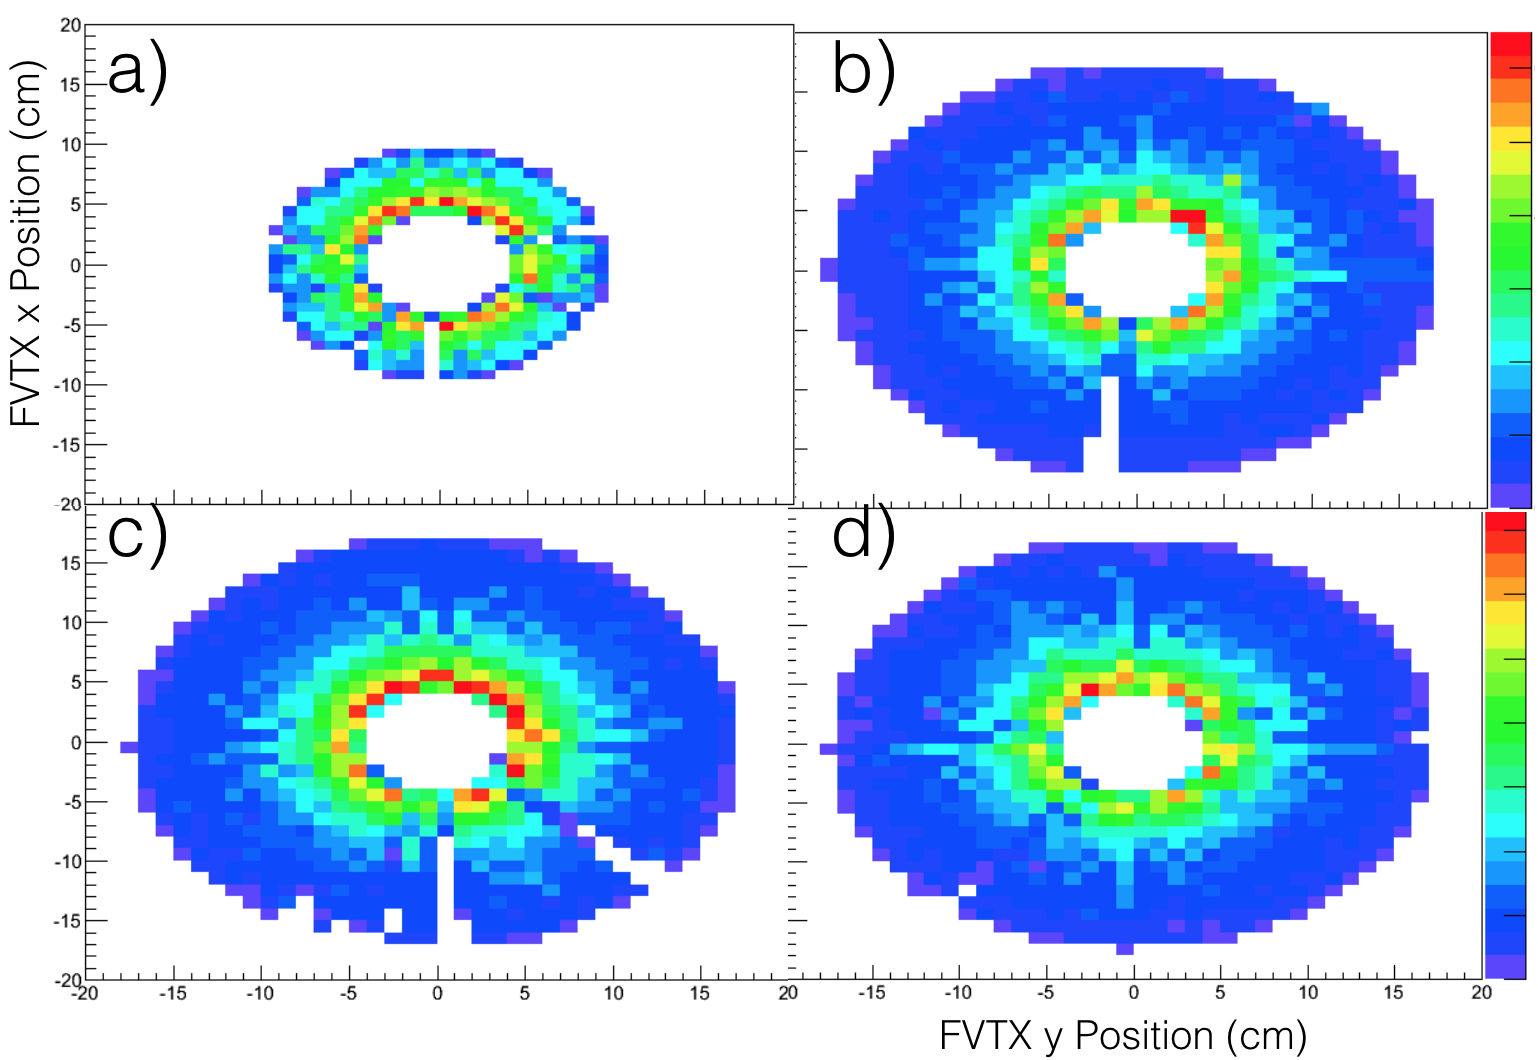
\includegraphics[width=0.55\linewidth]{figs/fvtx_clus_xy.png}
\caption{Distribution of FVTX clusters in $x$ and $y$ for layers 1, 2, 3, and 4 for panels a), b), c), and d), respectively. The color scale corresponds to the number of counts.}
\label{fig:fvtx_clusxy}
\end{figure}

\subsection{BBC PMTs}
The BBC provides information on the position, time of arrival, and number of charged particles that hit the BBC's quartz radiator material. The BBC acceptance is $3.1 < |\eta| < 3.9$ and spans the full azimuth. The resolution of the detector in $x$ and $y$ is 5 cm, corresponding to the diameter of a BBC PMT. In addition to spatial information, the BBC provides charge information, calibrated so that a value of 1.0 corresponds to a single charged particle hitting the detector (i.e. one minimum ionizing particle traversing the quartz). Figure \ref{fig:bbc_rings} shows the layout of the PMTs for the BBC. As discussed in section \ref{sec:bbc_det_sec}, the information regarding arrival time and particle charge can be used to calculate the $z$-vertex of the collision. 
\begin{figure}[!ht]
\centering
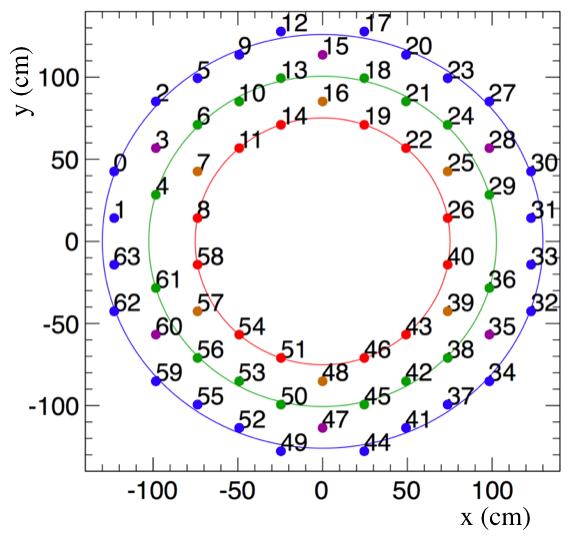
\includegraphics[width=0.55\linewidth]{figs/bbc_rings.png}
\caption{Diagram showing the positions of the PMTs for the south BBC detector. Rings shown with the same color indicate PMTs at an approximate common radius.}
\label{fig:bbc_rings}
\end{figure}

%\section{Two-particles Correlation}
%\subsection{Measurement in \pp and \pau}

\section{The Event Plane Method}
Details of the event plane method were given in Chapter 2 Section \ref{sec:event_plane}.
The goal of this thesis is to measure $v_2$, which is related to collective behavior as evidenced by correlations among particles. These correlations exist relative to the orientation of the collision. The event plane method measures the azimuthal anisotropy in final state particles. The event plane method uses final state particles to calculate the event plane angle from the data. A different set of final state particles are used to define the event plane in the FVTX or BBC and measure the $v_2$ in the CA. 

An event plane angle is defined for each harmonic, and is denoted as $\Psi_n$ where $n$ is the harmonic number. The definition for $\Psi_n$ is related to the calculation of the Q-vector. For an event with $N$ particles, define the flow vector $\vec{Q}$ as follows:

\begin{align}
Q_x &= \sum_{i=1}^{N}( w_i \cos(n \phi_i)) \\
Q_y &= \sum_{i=1}^{N}( w_i \sin(n \phi_i)) \\
Q_w &= \sum_{i=1}^{N}( w_i )
%\Psi_n &= \arctan( \frac{Q_y}{Q_x} ),
\label{eqn:general_ep_math}
\end{align}
where $i$ is the $i$th particle in the event, $\phi_i$ is the azimuthal angle of the particle, $w_i$ is the weight factor, and $n$ is the harmonic number. We define the $n$th order event plane as
$\Psi_n = \arctan \left( \frac{Q_y}{Q_x} \right). $

Once the event plane has been calculated, the flow harmonics ($v_n$) are defined as
\begin{equation}
v_n = \frac{\langle \langle\cos(n(\phi - \Psi_n))\rangle \rangle}{Res(\Psi_n)},
\end{equation}
where $\langle \langle \rangle \rangle$ indicates that $\cos(2(\phi-\Psi_n))$ is averaged over all particles in the same event, and the resulting $v_2$ must be averaged over many events \cite{PhysRevC.58.1671}. Note, the event plane angle and the Q-vector are defined at the event level.
  
As discussed in Chapter 2, Section \ref{sec:event_plane}, the event plane angle is a measurement which attempts to correspond to the physical participant plane angle. Thus, the event plane is an imperfect representation of the reaction plane and needs to be corrected. This correction is known as the event plane resolution $Res(\Psi_n)$, and is calculated using the 3-subevent method. It is important to note the set of particles used to calculate $\Psi_n$ and $\phi$ must be different in order to avoid autocorrelations. This is usually done by imposing an $\eta$ gap (at least a half of a unit of pseudorapidity)between the two particle sets.

For this analysis, the event plane is calculated separately for each of the forward detectors mentioned above, i.e., the BBC and the FVTX. We only use the south (Au-going) side of each detector, referred to here as the BBCS and the FVTXS.
For the FVTXS, the Q-vector is calculated in each event as
\begin{align}
Q_x &= \sum^{N_{\rm cluster}}_{i=1}( \cos(n\phi_i)) \\
Q_y &= \sum^{N_{\rm cluster}}_{i=1}( \sin(n\phi_i)) \\
\phi_i &= \arctan\left(\frac{y^i_{\rm cluster}}{x^i_{\rm cluster}}\right)
\end{align}
where $N_{\rm cluster}$ is the number FVTXS clusters in that event and $x^i_cluster$ and $y^i_cluster$are the $x$ and $y$ components of the $i$th FVTXS cluster in that event. At this point, this Q-vector is calculated with no cluster dependent weight factor because each cluster is taken to be the representation of one particle in each layer.

For the BBCS, the Q-vector is calculated in each event as
\begin{align}
Q_x &= \sum^{N_{\rm PMT}}_{i=1}( w_i \cos(n\phi_i)) \\
Q_y &= \sum^{N_{\rm PMT}}_{i=1}( w_i \sin(n\phi_i)) \\
Q_w &= \sum^{N_{\rm PMT}}_{i=1}( w_i ) \\
\phi_i &= \arctan\left(\frac{y^i_{\rm PMT}}{x^i_{\rm PMT}}\right) 
\label{eqn:bbc_ep_eqns}
\end{align}
where $w_i$ is the scaled charge collected on the PMT and $N_{\rm PMT}$ is the number of PMTs that fired (above threshold) in each event.

Finally, the $v_n$ are calculated using a combination of the BBCS or FVTX Q-vectors and the CA tracks as
\begin{equation}
v_n = \frac{\left<\left<\cos(n(\phi^{CA} - \Psi^{BBCS,FVTXS}_n))\right>\right>}{Res(\Psi^{BBCS,FVTXS}_n)}.
\end{equation}
In this analysis, we are concerned only with measuring the second-order harmonic $v_2$.

\subsection{Event Plane Resolution Calculation}%bulk up this section with more background
As mentioned above, the event plane resolution is calculated using the standard 3-subevent method~\cite{PhysRevC.58.1671}. The strategy of this method is to measure $\Psi_2$ with three different detectors in the same event, and then algebraically. The event plane resolution is defined as
\begin{equation}
Res(\Psi_2^A) = \sqrt{\frac{\left<\cos(2(\Psi_2^A - \Psi_2^B))\right>\left<\cos(2(\Psi_2^A - \Psi_2^C))\right>}{\left<\cos(2(\Psi_2^B - \Psi_2^C))\right>}},
\label{eqn:res}
\end{equation}
where A,B, and C are three detectors measuring the same event. Here, the term ``subevent'' refers to the specific subset of particles measured by a given detector~\cite{PhysRevC.58.1671}.

\begin{figure}[!h]
\centering
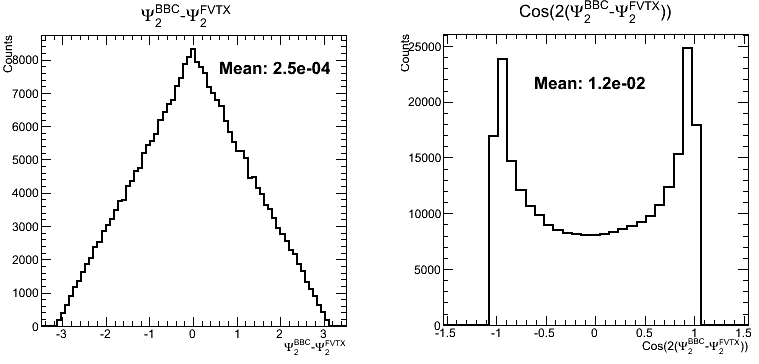
\includegraphics[width=0.75\linewidth]{figs/resolution_intermediate_calc.png}
\caption{Intermediate steps involved in calculating the event resolution. Raw difference between the event plane angles for two different detectors (left). This distribution is triangular because it is the result the cross-correlation of two nearly uniform distributions, $\Psi_2^{\rm FVTXS}$ and $\Psi_2^{\rm BBCS}$. The cosine of two times the difference between the two event plane angles. The average of this distribution is used in Equation \ref{eqn:res} (right).}
\label{fig:res_interm_calc}
\end{figure}

In this analysis, the three detectors used to provide the required three subevents are the FVTX-south, the BBC-south, and the CA, which span pseudorapidity acceptances of $-3 <\eta < -1$, $-3.9 < \eta < 3.1$, and $|\eta| < 0.35$, respectively. Figure \ref{fig:res_interm_calc} shows the event-by-event relative difference of $\Psi_2^{\rm BBCS}$ and $\Psi_2^{\rm FVTXS}$. Unlike the BBCS and the FVTXS, the CA detector does not have full azimuthal acceptance coverage. Therefore, the event plane angle cannot be reliably calculated with this detector for events whose event plane points outside of the acceptance. In order to solve this problem, we calculate the event plane resolution using a different, yet mathematically equivalent formulation that does not make use of $\Psi^{\rm CA}$, as given below for the $\Psi^{\rm FVTXS}$:

%However, due to the fact that the CNT detector does not have full azimuthal coverage, the CNT event plane is not well defined for a class of events where the event plane doesn't point into the CNT acceptance, therefore the event plane resolution is calculated via a modified yet mathematically equivalent definition to the one mentioned above. This modified method allows the resolution of the FVTX-S and the BBC-S to be calculated using the CNT without having to calculate CNT event plane. It is defined as
\begin{equation}
Res(\Psi_n^{\rm FVTXS}) = \sqrt{\frac{\left<\left<\cos(n(\Psi_n^{\rm FVTXS} - \phi^{CA}))\right>\right>\left<\cos(n(\Psi_n^{\rm FVTXS} - \Psi_n^{\rm BBCS}))\right>}{\left<\left<\cos(n(\phi^{CA} - \Psi_n^{\rm BBCS}))\right>\right>}},
\end{equation}
where there is a double average over each CA track and each event.
\begin{table}[!ht]
\caption{The event plane angle resolutions for the FVTXS and the BBCS for the second and third order harmonics.}
\begin{center}
    \begin{tabular}{| l | l | l | l |}
    \hline
    Detector & $n=2$ & $n=3$  \\ \hline
    FVTXS & 0.216 & 0.010 \\ \hline
    BBCS & 0.052 & 0.010  \\ \hline
    \end{tabular}
\end{center}
\label{tbl:std_resolutions}
\end{table}

\subsection{Event Plane Flattening Calibration}
In order for the event plane to be useful in making a $v_n$ measurement, the event plane angle must be calibrated such that its distribution is uniform. For the event plane method, a physical assumption is made that the true distribution of $\Psi_n$ angles will be uniform since physically there is no preferred orientation of the collision. If the measured $\Psi_n$ distribution is not flat, we attribute that behavior to variations in the efficiency of detecting charged particles as a function of $\phi$. Thus, the event plane calibration procedure seeks to correct for these non-uniformities in acceptance, and restore the $\Psi_n$ distribution to the physical expectation of uniformity. We employ a procedure to re-center and flatten the measured non-uniform $\Psi_n$ distribution.

%\begin{figure}[htbp]
%\begin{center}
%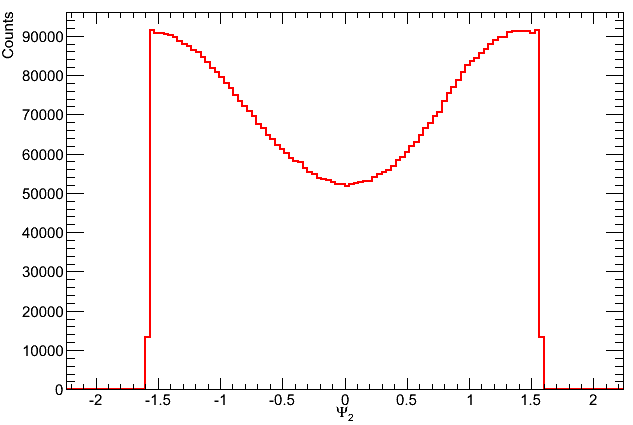
\includegraphics[width=0.65\linewidth]{figs/example_raw_psi2.png}
%\caption{This is the BBC-S $\Psi_2$ distribution before any calibration. The range of the $\Psi_2$ resolution is from $\frac{-\pi}{2}$ to $\frac{\pi}{2}$ because of the periodicity. 
%The raw distribution has a sinusoidal shape.}
%\end{center}
%\label{fig:raw_psi}
%\end{figure}

Figure~\ref{fig:calibrated_psi} shows an example of $\Psi_2$ distributions for the BBCS at the different stages of the calibration. The raw $\Psi_2$ (shown in red) has a significant deviation from uniformity which needs to be corrected. The flattening calibration attempts to correct for this lack of uniformity by shifting the $\Psi_2$ value of each individual event by an amount corresponding to the deviation of the overall distribution for all events. Although this procedure results in a uniform $\Psi_2$ distribution, applying too large of a correction arising from an exceedingly distorted initial distribution can lead to systematic effects on the $v_2$ measurement, which will be discussed in the next section. Therefore, it is important to address any systematic effects that would affect the uniformity of the $\Psi_2$ distribution.
\begin{figure}[!h]
\centering
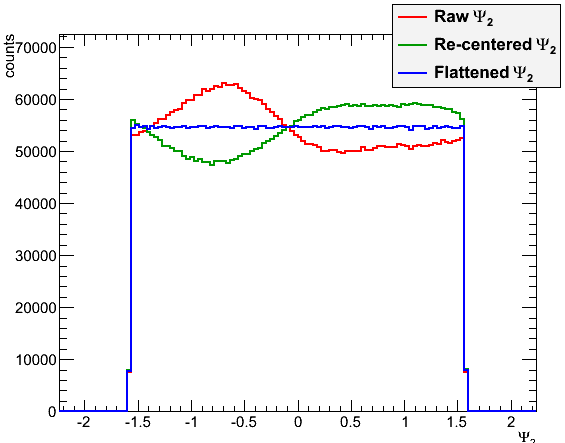
\includegraphics[width=0.65\linewidth]{figs/flattened_example_fvtx.png}
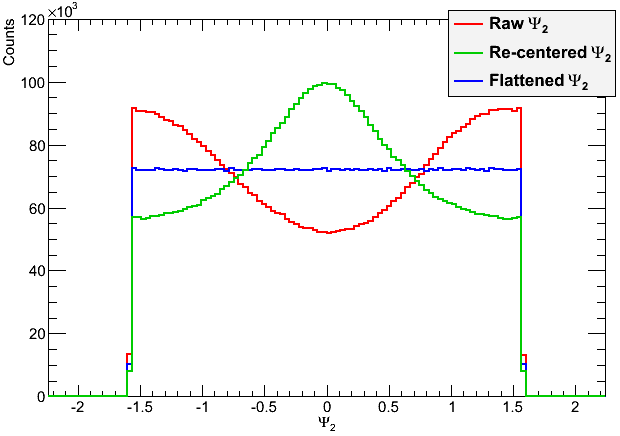
\includegraphics[width=0.62\linewidth]{figs/flattened_example_bbc.png}
\caption{This is the $\Psi_2$ distribution projected over all z-vertex bins at different steps during the calibration. The top is from the FVTX south and the bottom is from the BBC south. The range of the $\Psi_2$ resolution is from -$\frac{\pi}{2}$ to $\frac{\pi}{2}$ because of the periodicity. The raw (in red) $\Psi_2$ distribution has a sinusoidal shape. The re-centered (in green) $\Psi_2$ distribution moves the mean. The flattened (in blue) $\Psi_2$ distribution spreads out the counts so that there is uniformity. Each calibration step preserves the integral.}
\label{fig:calibrated_psi}
\end{figure}

The flattening calibration requires two steps to completely flatten the $\Psi_n$ distribution. The first step of the calibration is to re-center the mean of the raw $\Psi_n$ distribution. The second step is to Fourier transform the re-centered distribution and use the transformation to shift the $\Psi_n$ values to a uniform distribution. With flattening, each $\Psi_n$ is transformed to $\Psi_n + \Delta\Psi_n$. $\Delta\Psi_n$ is defined as
\begin{equation}
\Delta\Psi_n = \sum^{N}_{i=1}\left(\frac{2}{i}\left(\sin(i \Psi)F^{\cos}_{i}(f(\Psi_n))-\cos(i \Psi)F^{\sin}_{i}(f(\Psi_n)\right)\right),
\label{eq:deltapsi}
\end{equation}
where $N$ is the number of components, $F^{\cos}_{i}(f(x))$ is the $i$th component of the cosine Fourier transform of $f(x)$, and $f(\Psi_n)$ is the $\Psi_n$ distribution. For this analysis, $N = $12 is a sufficient number of components to flatten the $\Psi_n$ distribution. The re-centering and flattening calibration is done in separate 30 $z$-vertex bins since the detector acceptance in $\phi$ will vary with z-vertex.

\section{East West $v_2$ Discrepancy}
As discussed in the previous section, distortions in the raw $\Psi_2$ distribution can cause distortions in the measurement of $v_2$. In this section, we discuss how the beam alignment effects the raw $\Psi-2$ distribution and how it can be corrected for.
\begin{figure}[!h]
\centering
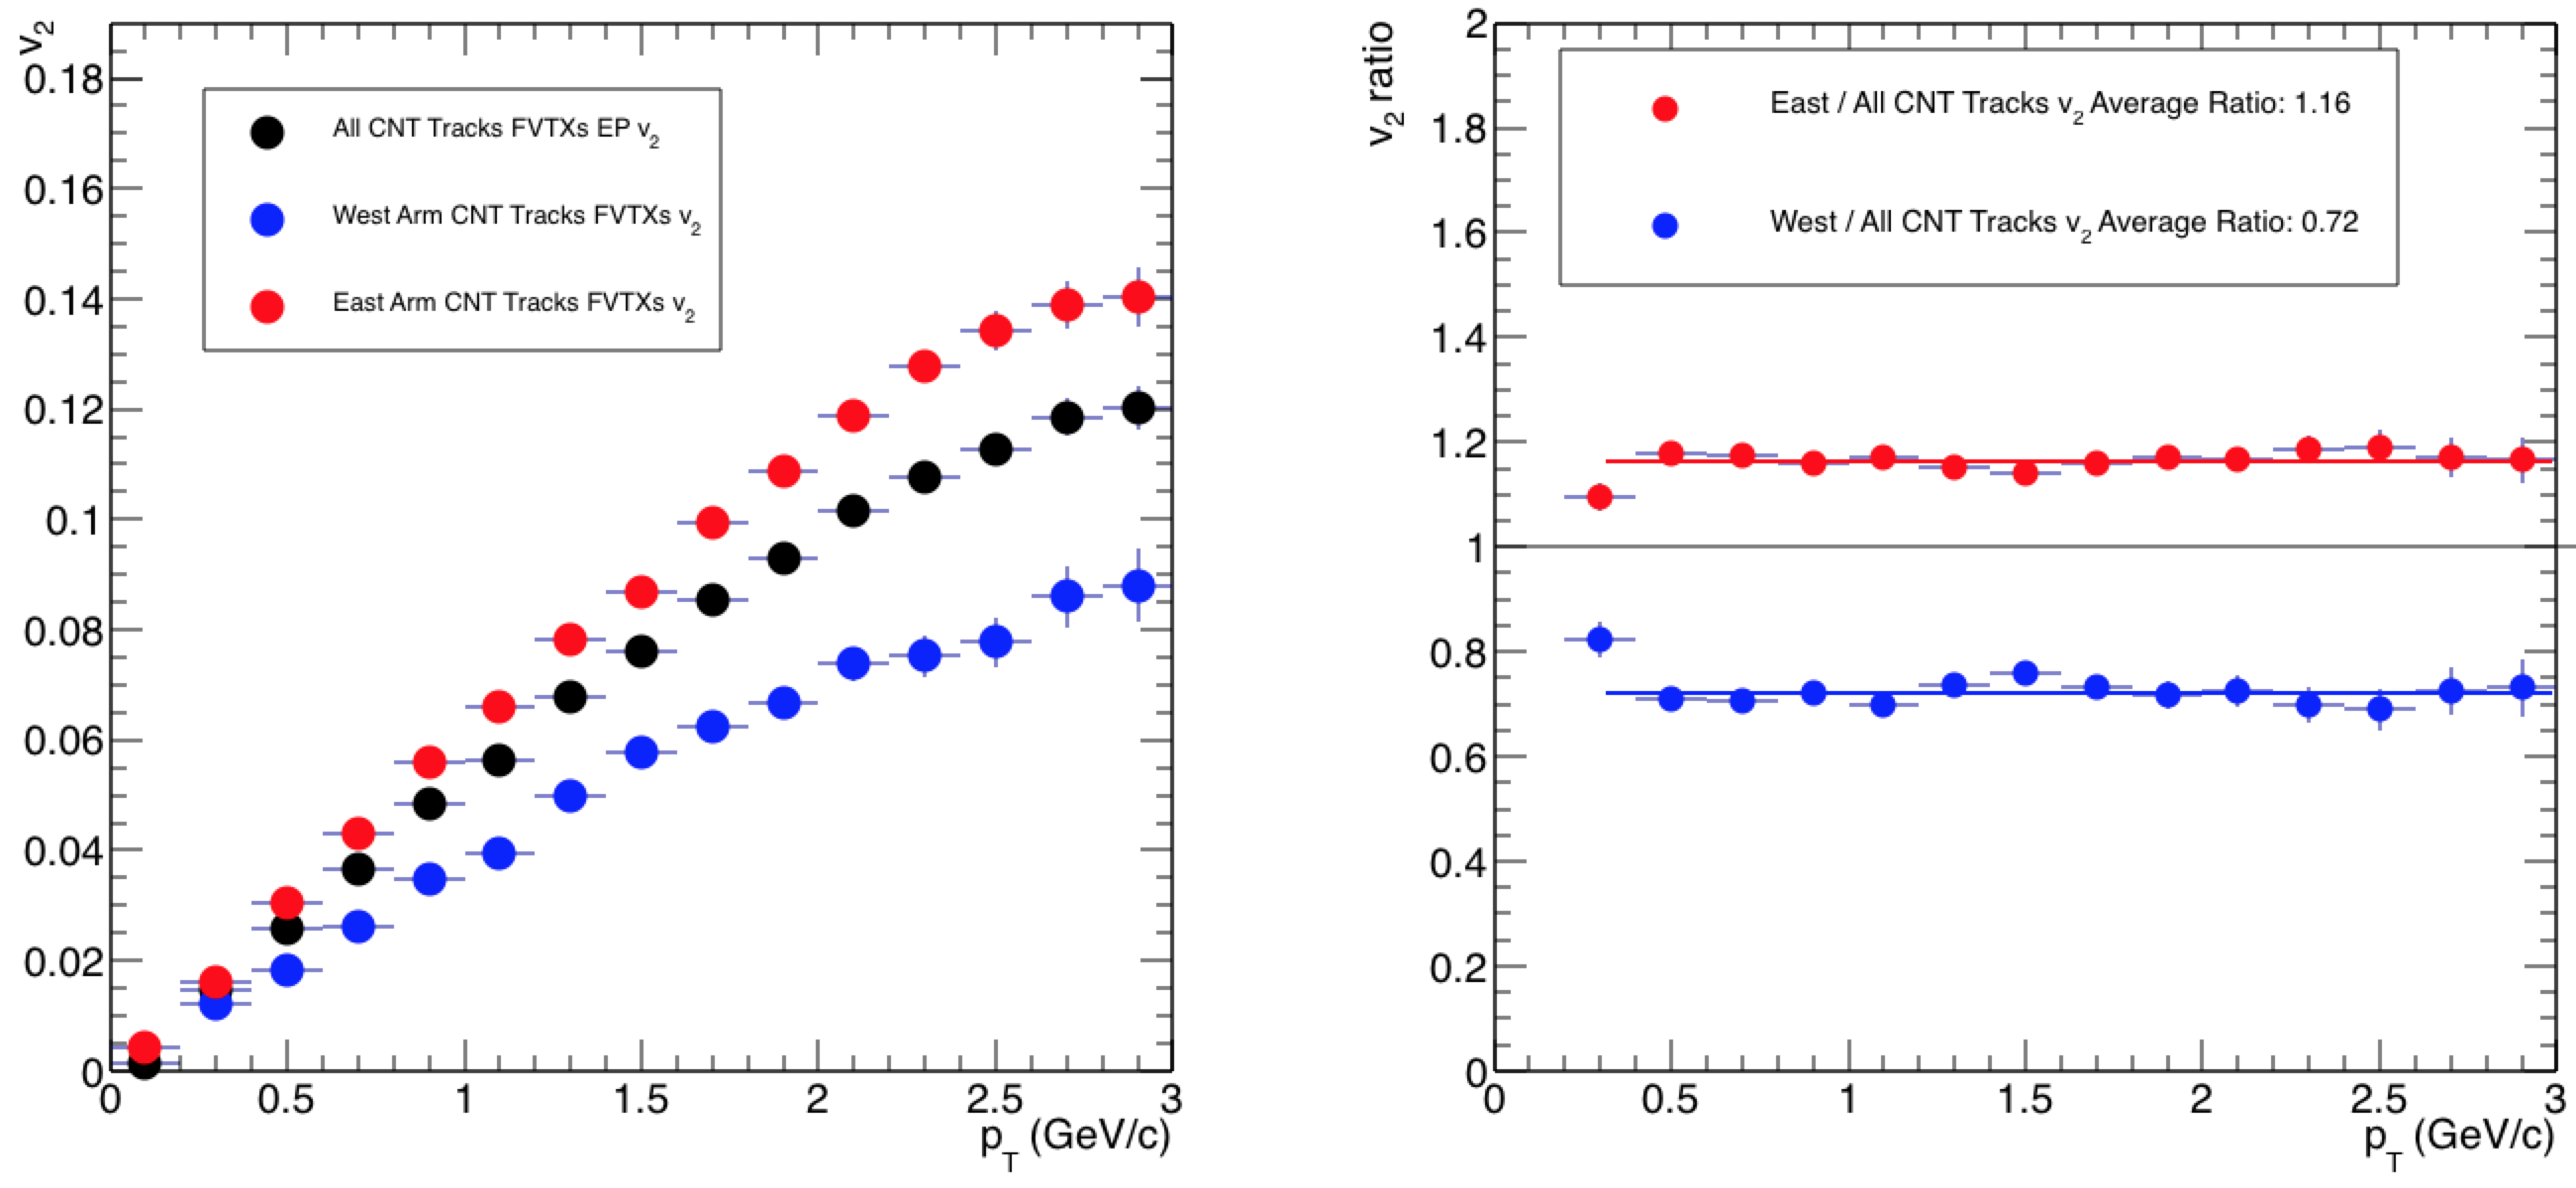
\includegraphics[width=0.85\linewidth]{figs/fvtxs_default_ew.png}
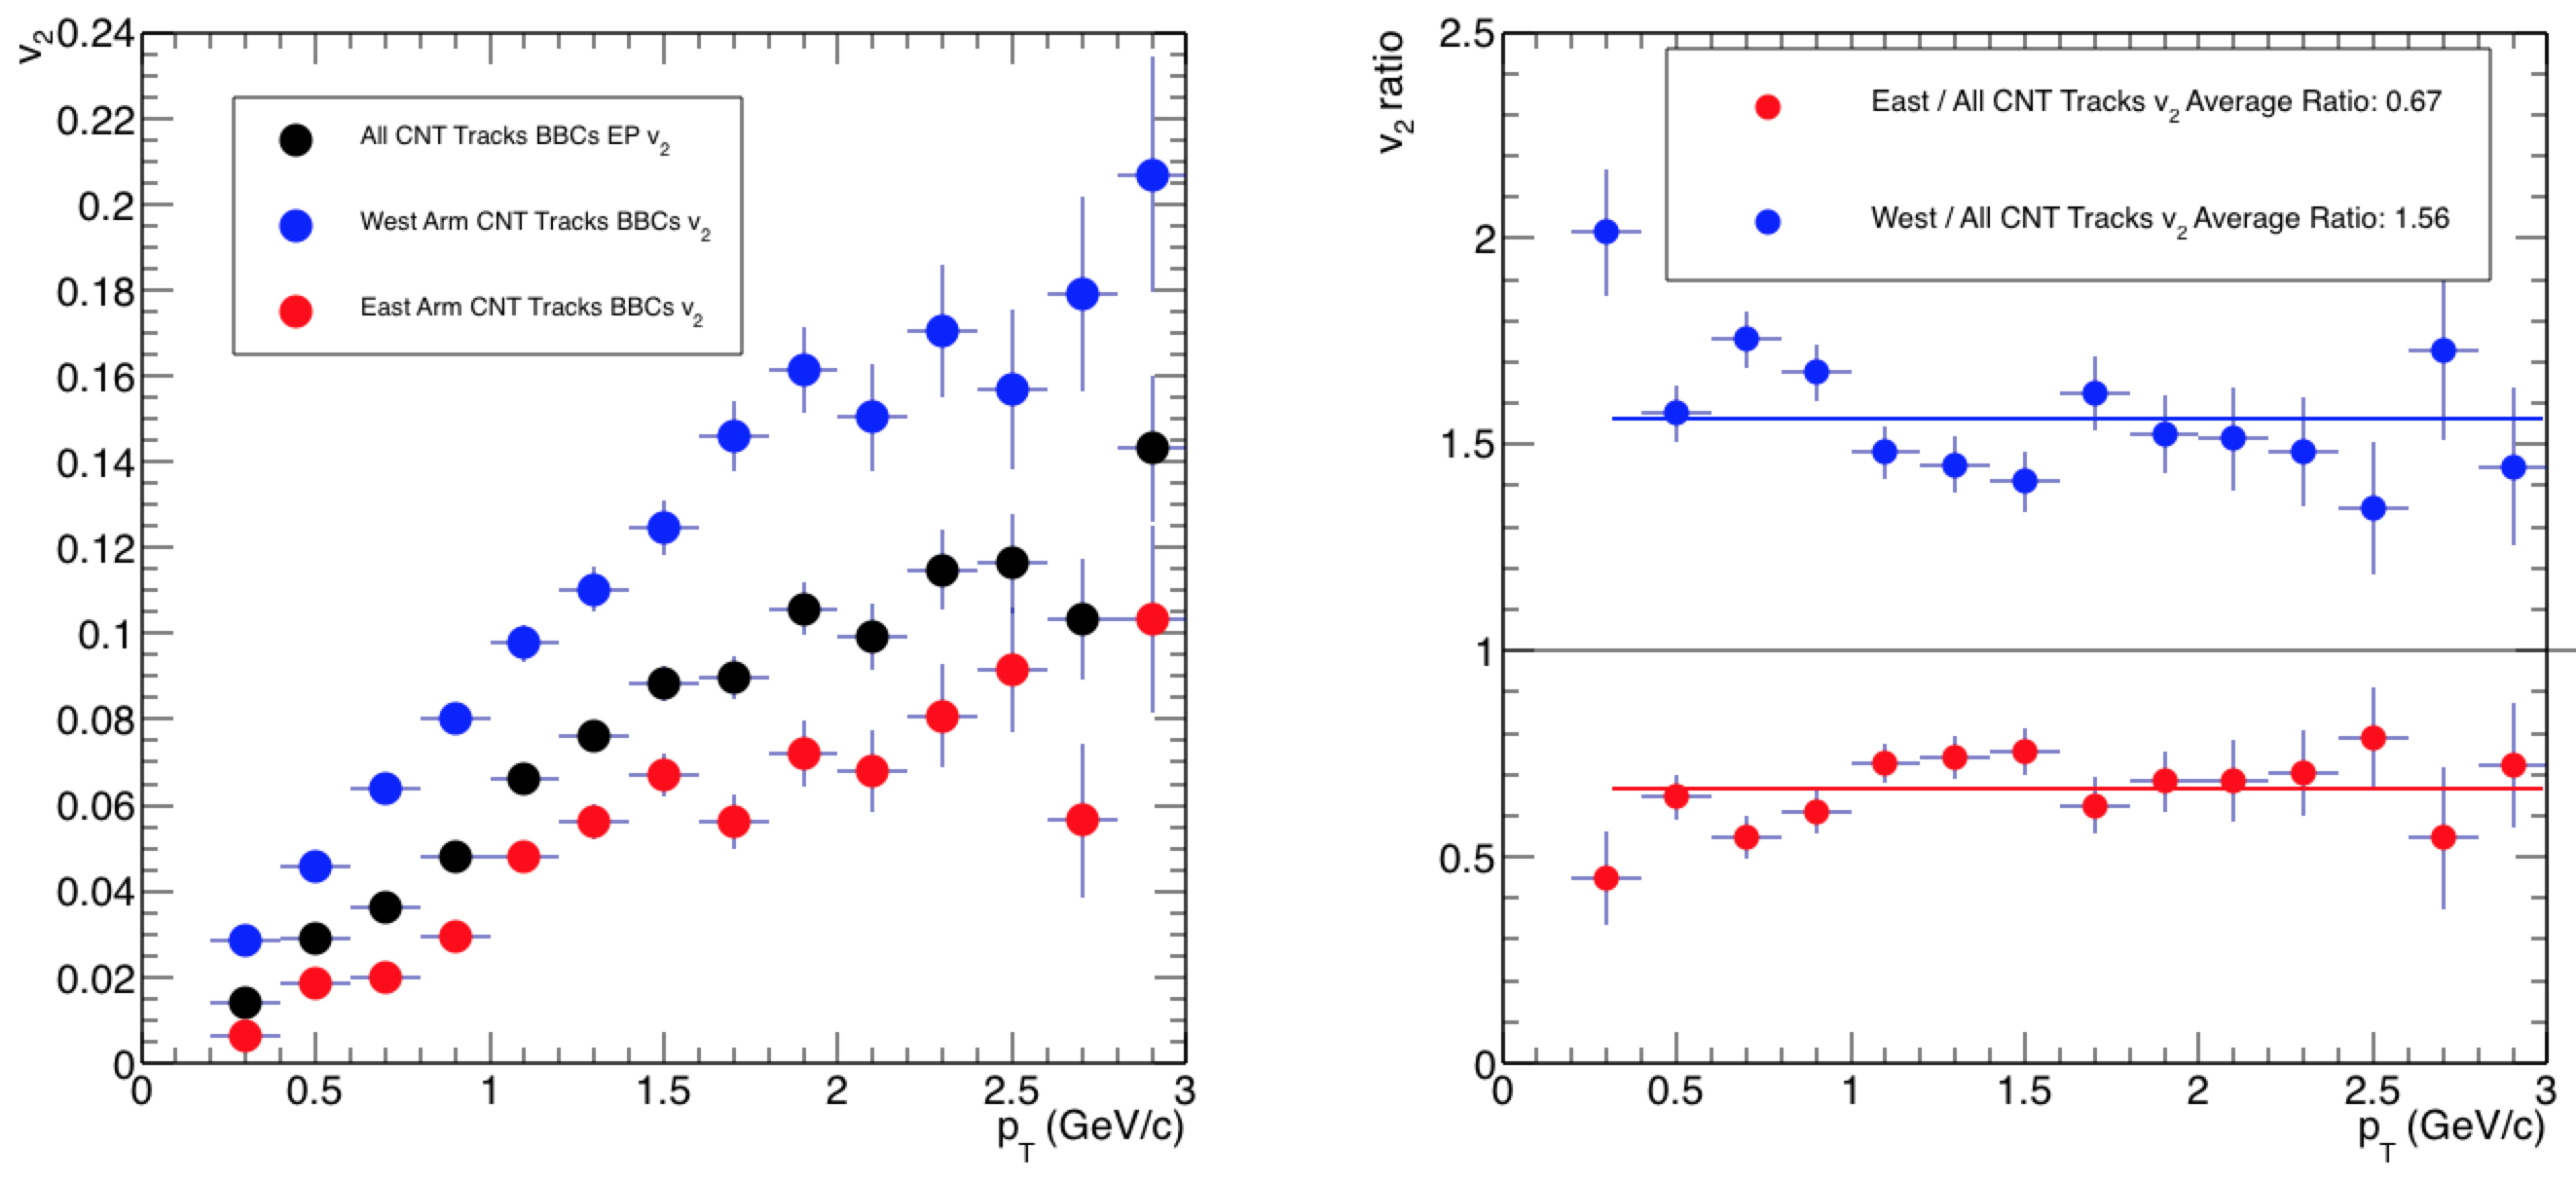
\includegraphics[width=0.85\linewidth]{figs/bbcs_default_ew.png}
\caption{First attempt at measuring $v_{2} (p_T)$ with the event plane as calculated with the FVTXS (top left) and the BBCS (bottom left) in the \pau at \sqsn = 200 GeV dataset, using the default resolution as shown in Table \ref{tbl:std_resolutions}. The black points show $v_2$ measured using all CA tracks. The blue and red points show $v_2$ measured using only tracks in the west and east arms, respectively. The ratios are fit with a constant, whose value is shown in the legend.}
\label{fig:fvtx_ew_default}
\end{figure}

As shown in Figure~\ref{fig:fvtx_ew_default}, $v_2$ is different when measured using tracks in the west (-1 $<$ $\phi$ $<$ 1) and east arm (2 $<$ $\phi$ $<$ 4) of the CA. This is a systematic effect explained by the colliding beams not being parallel to the longitudinal axis of PHENIX. When examining beam alignment effects on the $v_2$ measurement, we can quantify the east-west $v_2$ asymmetry by calculating $R_{v_2}$ which is calculated by: 
\begin{equation}
R_{v_2} = \frac{\int{v_2^{\rm east}(p_T)d\pt}}{\int{v_2^{\rm west}(p_T)d\pt}}.
\end{equation}
In Figure \ref{fig:fvtx_ew_default}, $R_{v_2^{\rm FVTXS}}$ can be extracted by taking the ratio of the numbers in the legend of the upper right plot and $R_{v_2^{\rm BBCS}}$ can be extracted the same way for the numbers in the bottom left plot's legend. The $R_{v_2^{\rm FVTXS}}$ = 1.61 while the $R_{v_2^{\rm BBCS}}$ = 0.43, indicating large east west asymmetry in both measurements, although the difference in the BBCS is bigger. It is interesting to note that the splitting of the east and west $v_2$ measurements goes in opposite directions for the BBCS as compared to the FVTXS. To understand where the discrepancy in these $v_2$ measurements comes from, we examine the effects of the beam alignment on the $v_2$ measurement.
\section{Correcting for the Effects of Beam Alignment}
As discussed in Chapter 3, Section \ref{sec:ch2_beam_col_geo}, due to the nature of running \pau at \sqsn = 200 GeV at RHIC, the beam geometry was not in accordance with the PHENIX coordinate system. First of all, the collision vertex is significantly offset from the z-axis to which all of the PHENIX detectors are aligned. The other beam geometry effect, and the more significant of the two effects, comes from the fact that the beams are colliding at an angle of 3.6 mRad in the x-z plane as show in Figure~\ref{fig:diagram2}~\cite{BNL_Run15_Operations}. The reason a non-ideal beam geometry creates an east west $v_2$ measurement difference is because of the assumption that the ideal event plane angle is azimuthally isotropic during the event plane flattening calibration. In the translated and rotated frame where the beams are aligned with the z-axis the event plane distribution would be uniform, but in the lab frame the event plane distribution in $\phi$ would have regions of enhancement and reduction. The event plane flattening calibration algorithm restores a non-uniform distribution to a uniform one; however, if the true event plane distribution is non-uniform then forcing the measured distribution to be uniform produces a systematic offset.

\begin{figure}[!ht]
\centering
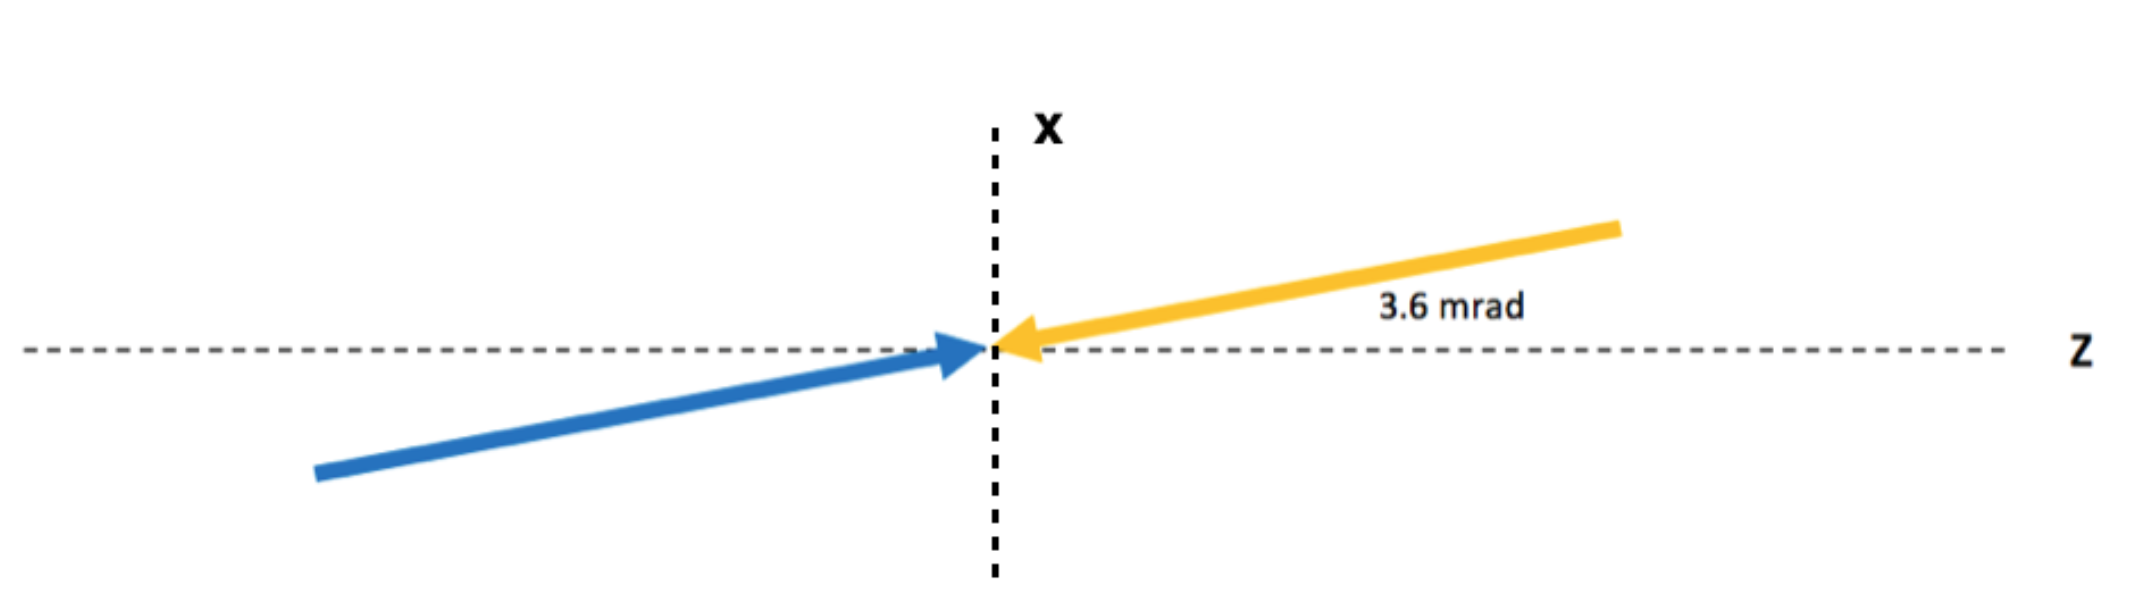
\includegraphics[width=0.75\linewidth]{figs/beam_angle.png}
\caption{Diagram illustrating the angle at which the yellow and blue beams collide relative to the longitudinal $z-$axis of the detector. The yellow beam corresponds to the Au (south-going) beam, and blue corresponds to the proton (north-going) beam. Due to the nature of running \pau collisions at \sqsn = 200 GeV at RHIC, the beams collide at an angle of 3.6 mrad.}
\label{fig:diagram2}
\end{figure}

We correct for the offset of the collision vertex by shifting the origin of the PHENIX global coordinate system to the true collision vertex. To correct for the effect of the beam angle, we apply a global rotation of the PHENIX coordinate to align its longitudinal axis with that of the beams. In practice, these transformations are accomplished by individually applying a global rotation and translation to every CA track, FVTX cluster, and BBC PMT. 

As shown in Figure~\ref{fig:fvtx_ew_rot}, applying these corrections prior to calculating $v_2$ reduces the magnitude of the east-west discrepancy. The new $R_{v_2^{\rm FVTXS}}$ = 1.43, and $R_{v_2^{\rm BBCS}}$ = 0.66, are reduced from the east-west difference measured without any corrections. However, even after rotating the PHENIX global coordinate system to be in alignment with the beam axis, $\Psi_2$ is, there is a residual effect from the beam rotation which still effects the $v_2$ measurement. 

\begin{figure}[!ht]
\centering
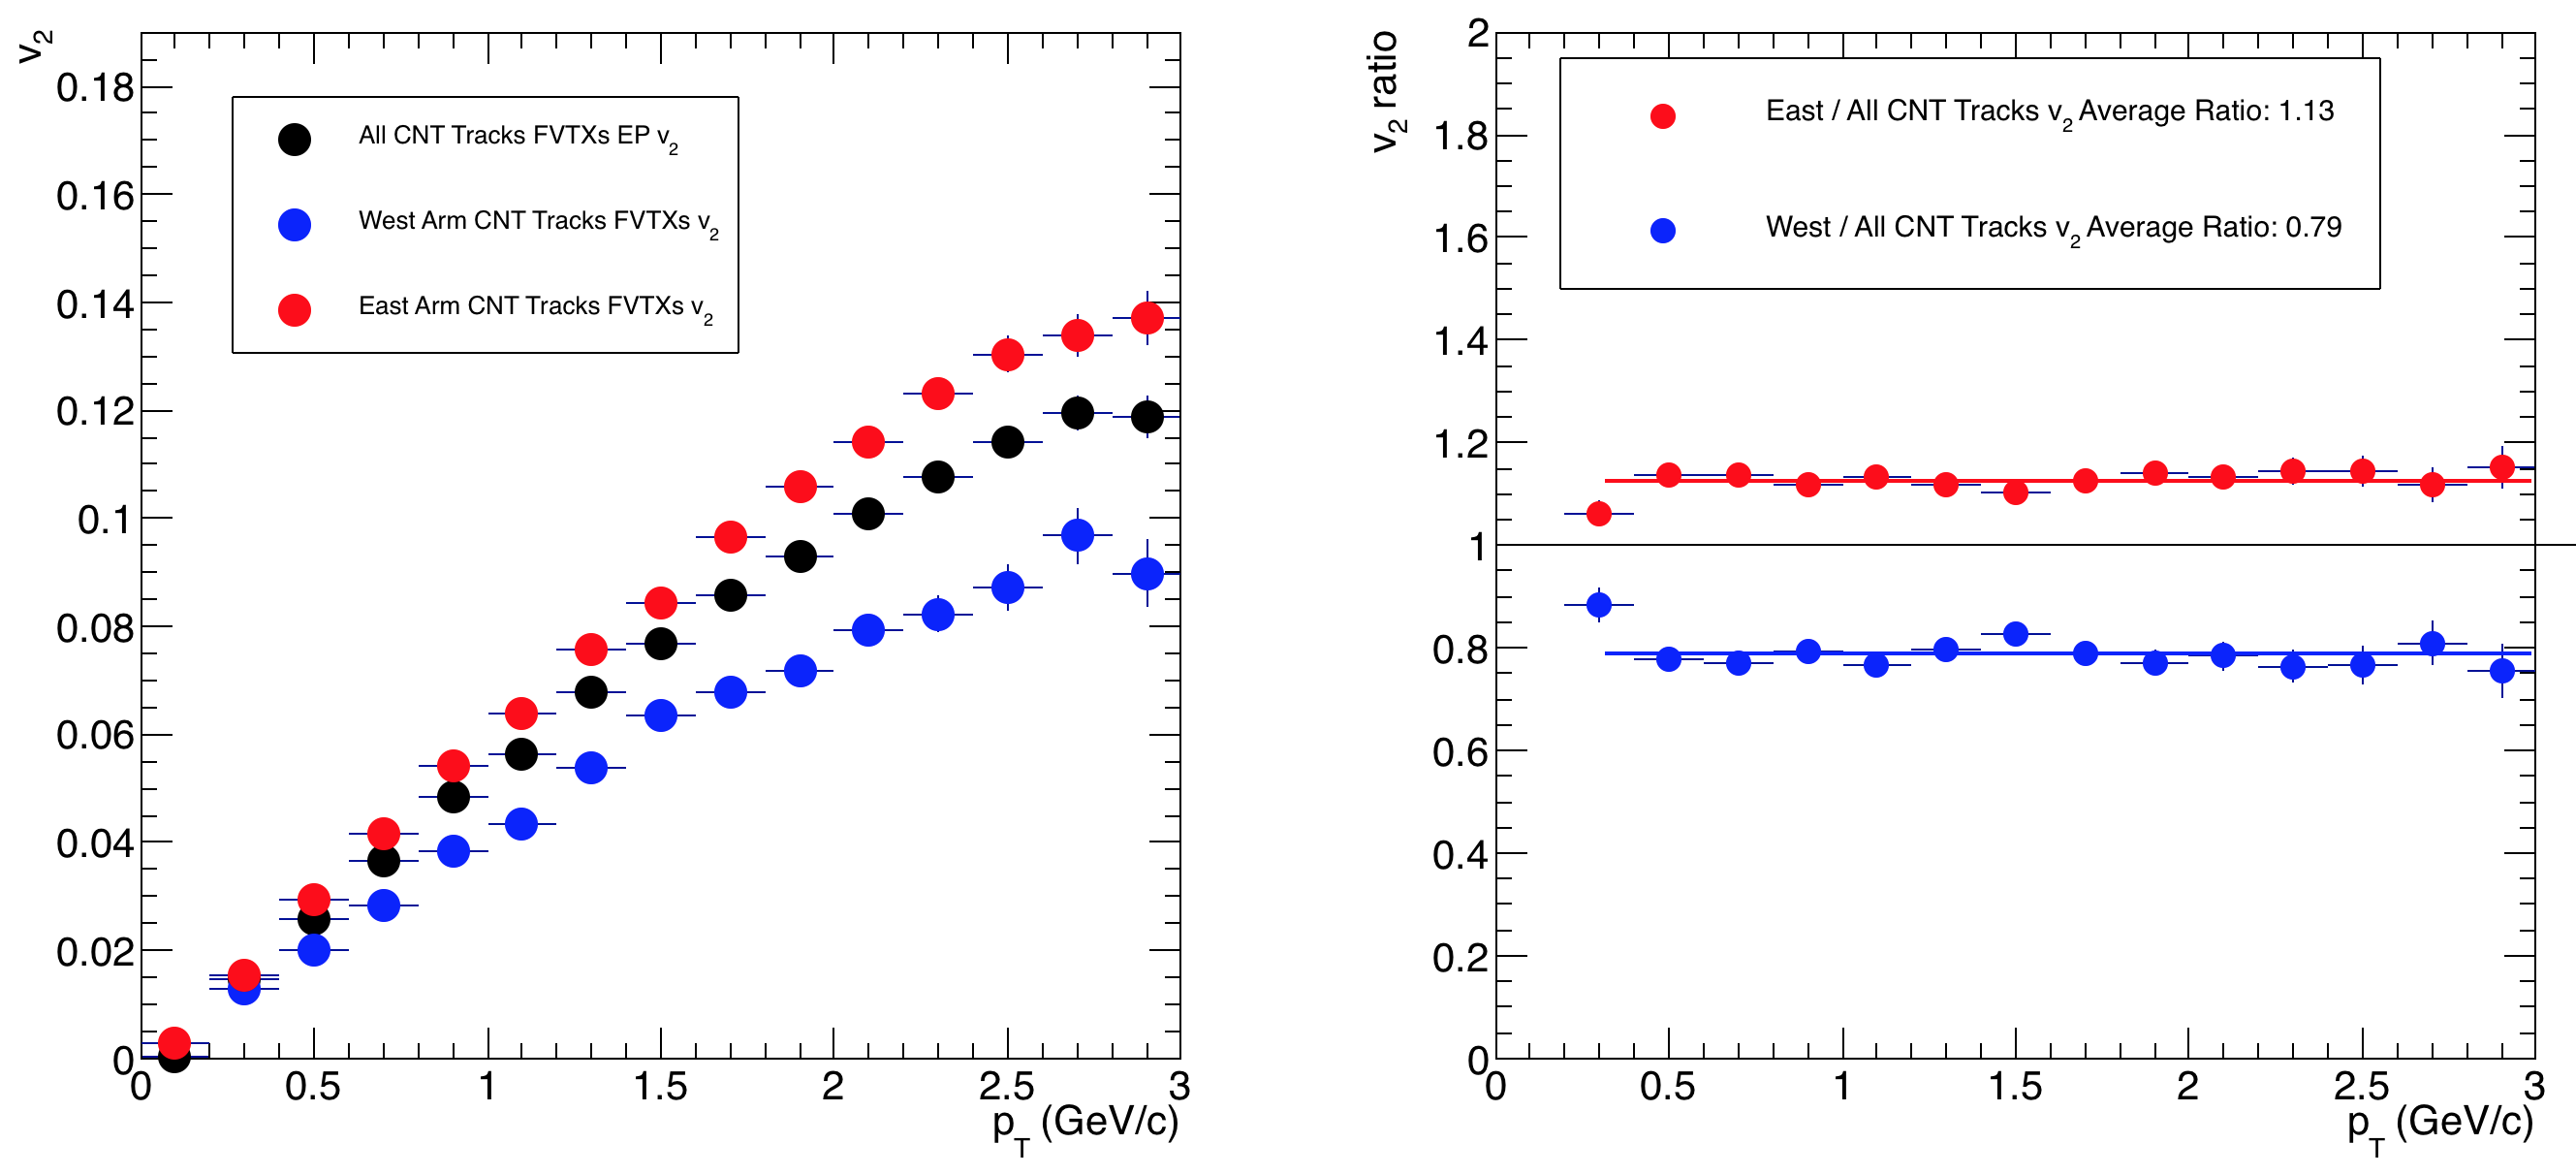
\includegraphics[width=0.85\linewidth]{figs/fvtx_vertex_rot_only.png}
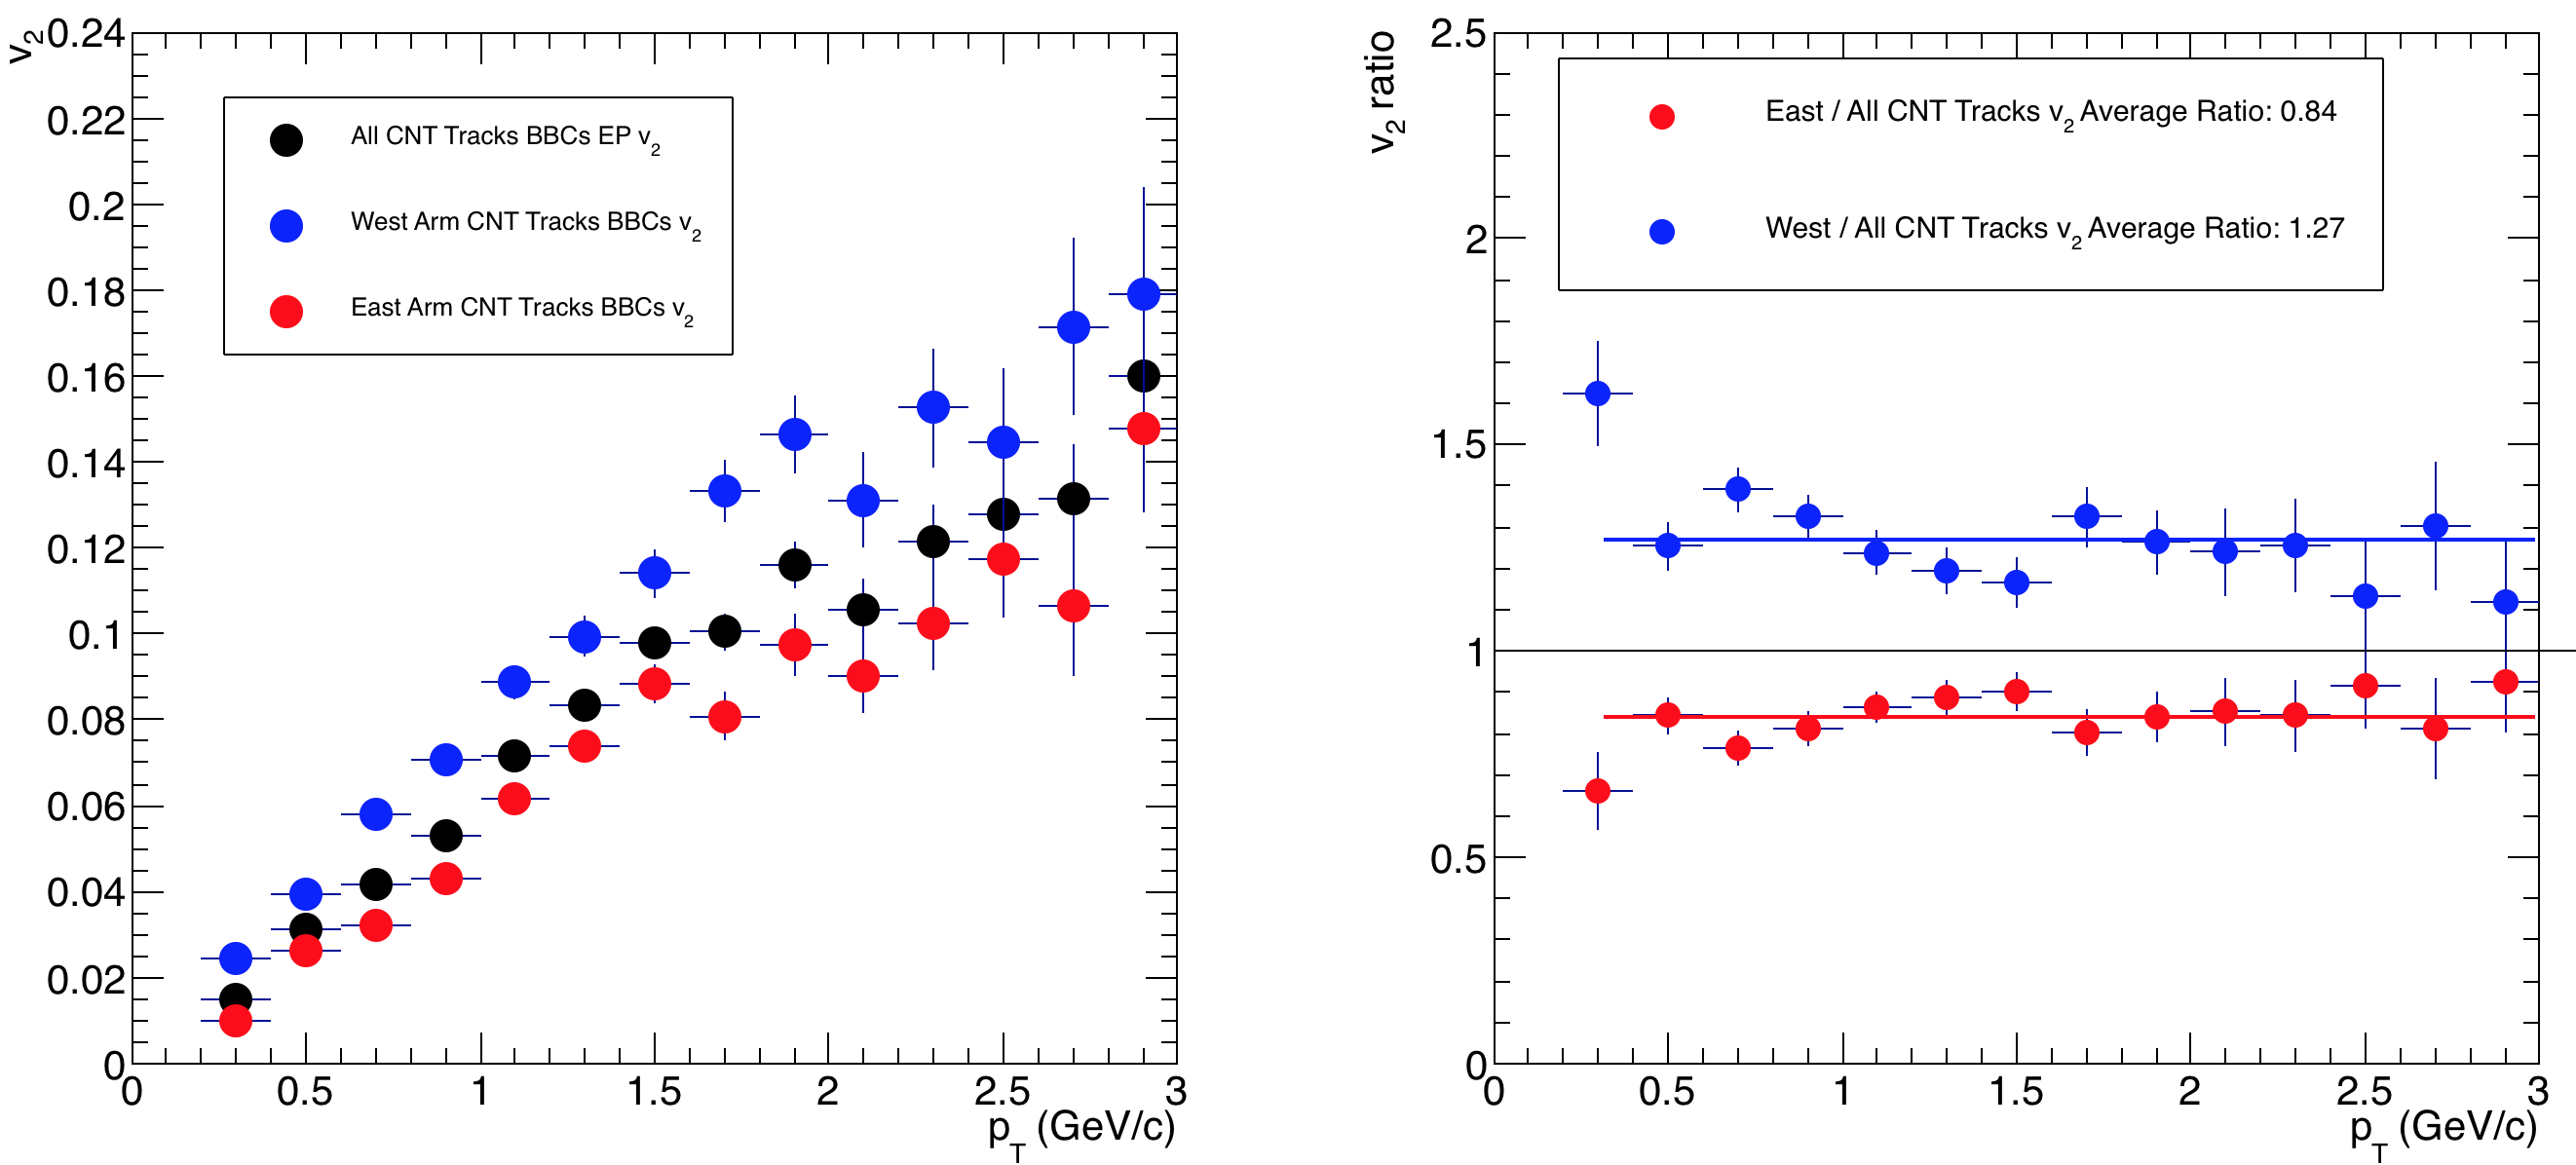
\includegraphics[width=0.85\linewidth]{figs/bbc_vertex_rot_only.png}
\caption{A corrected measurement of $v_{2}(\pt)$ with the FVTXS (top two panels) and the BBCS (bottom two panels) event plane for the \pau \sqsn = 200 GeV. The default resolution as shown in Table \ref{tbl:std_resolutions} is used. The plotting conventions are the same as described in the caption of Figure \ref{fig:fvtx_ew_default}. }
\label{fig:fvtx_ew_rot}
\end{figure}

To explain this effect, consider a cylindrical disk with a hole in the middle, centered about the z-axis (in analogy to the shape of the FVTX and the BBC), as shown in the left plot of Figure~\ref{fig:tilt_effect}. In this geometry, all points along a ring of constant radius are at the same pseudorapidity. However, if one were to tilt that disk, the pseudorapidity of points along that ring would be $\phi$ dependent. The tilt of the disk changes its pseudorapidity acceptance and its extent. Now consider that it is not the disk that is tilted but rather the beam orientation that is tilted. The previous statements about the effect on the $\eta$ range being $\phi$ dependent still apply. 

The combination of the $\eta$ acceptance changing and the $\eta$ distribution of charged particles not being flat means that the average number of charged particles going through the disk would be systematically $\phi$ dependent, as illustrated in Figure~\ref{fig:tilt_effect} (right). If the average charged particle distribution is not uniform in $\phi$, the event plane distribution will not be either. This results in the flattening procedure creating systematic effects such as the east-west $v_2$ asymmetry.

\begin{figure}[!ht]
\centering
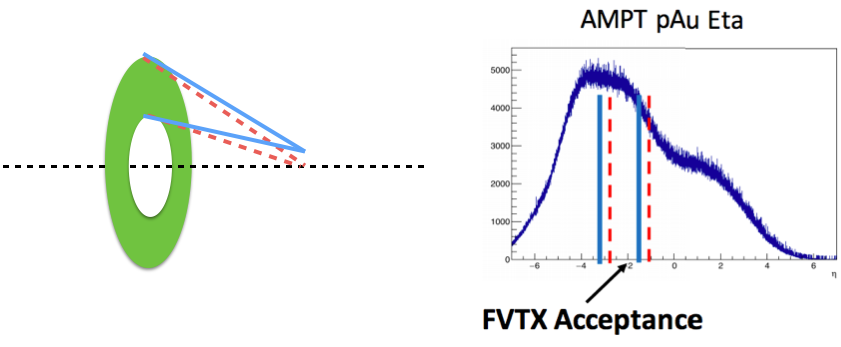
\includegraphics[width=0.95\linewidth]{figs/tilt_effect.png}
\caption{(left) Cartoon diagram illustrating $\eta$ acceptance shift due to a beam offset in one of the FVTXS layers. (right) Pseudorapidity distribution of charged particles from the AMPT Monte Carlo generator for \pau \sqsn = 200 GeV, showing the shift in $\eta$ acceptance.}
\label{fig:tilt_effect}
\end{figure}

In order to correct for this effect, an additional weight factor is introduced for FVTX clusters and BBC PMTs during the event plane calculation. This factor is such that hits in $\phi$ regions with systematically fewer particles are given a larger weight, and correspondingly, hits in $\phi$ regions with systematically more particles are weighted less. The introduction of this weighting as defined below does not formally change the event plane calculation, as a weight factor is already implemented in its construction. The modified weight factor is:
\begin{equation}
w_i = w^D_i F(\phi,z_{\rm vertex})
\label{eqn:modified_weight}
\end{equation}
where $w^D_i$ is the default weighting associated with the detector element, and $F(\phi,z_{\rm vertex})$ is the multiplicative weighting to correct for the beam geometry. $F(\phi,z_{\rm vertex})$ is dependent on $z_{\rm vertex}$, in addition to $\phi$, because $\eta$ is dependent on the collision vertex. 

\subsection{Analytic Correction Method}
One can analytically calculate this $\phi$ dependent weight factor using the geometry of the FVTXS and BBCS as well as using the $\eta$ distribution of charged particles. Unfortunately, the $\eta$ distribution of charged particles in \pau \sqsn = 200 GeV has not been measured by an experiment, so we must rely on models that cannot be fully checked. We can simulate 0--2 fm impact parameter \pau at \sqsn = 200 GeV events in AMPT and determine the simulated $dN_{ch}$/$d\eta$ as shown in the right panel of Figure \ref{fig:tilt_effect}. 

The left panel of Figure \ref{fig:analytic_corr} shows the $\phi$ dependence of the $\eta$ acceptance with a beam angle (solid line) and without a beam angle (dotted line). By taking the ratio of the $\eta$ acceptance with a beam angle to the $\eta$ acceptance without a beam angle, for each $\phi$ angle we calculate the correction factor shown in the right panel of Figure \ref{fig:analytic_corr}. This correction factor is the multiplicative weight factor $w_i$ as defined in the previous section.
\begin{figure}[!ht]
\centering
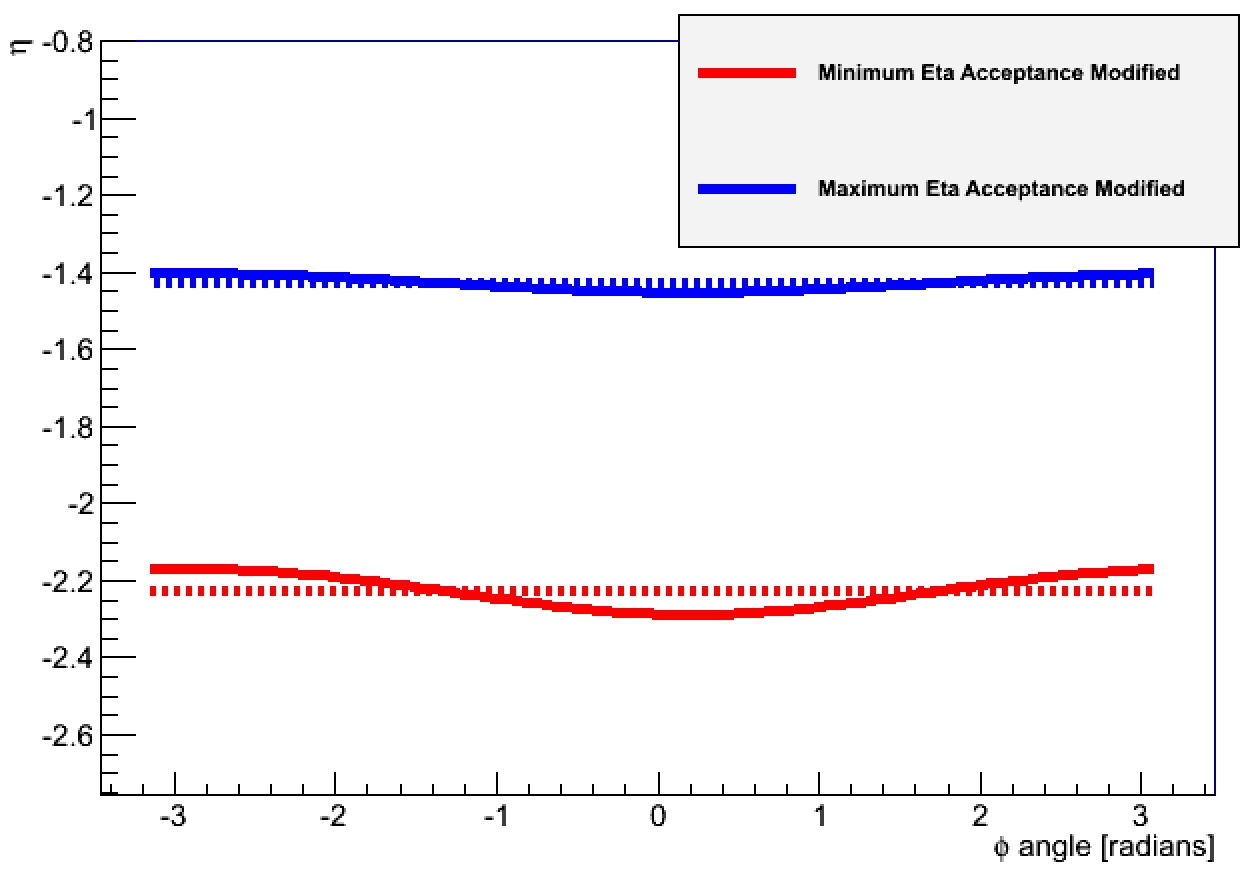
\includegraphics[width=0.47\linewidth]{figs/eta_modification.png}
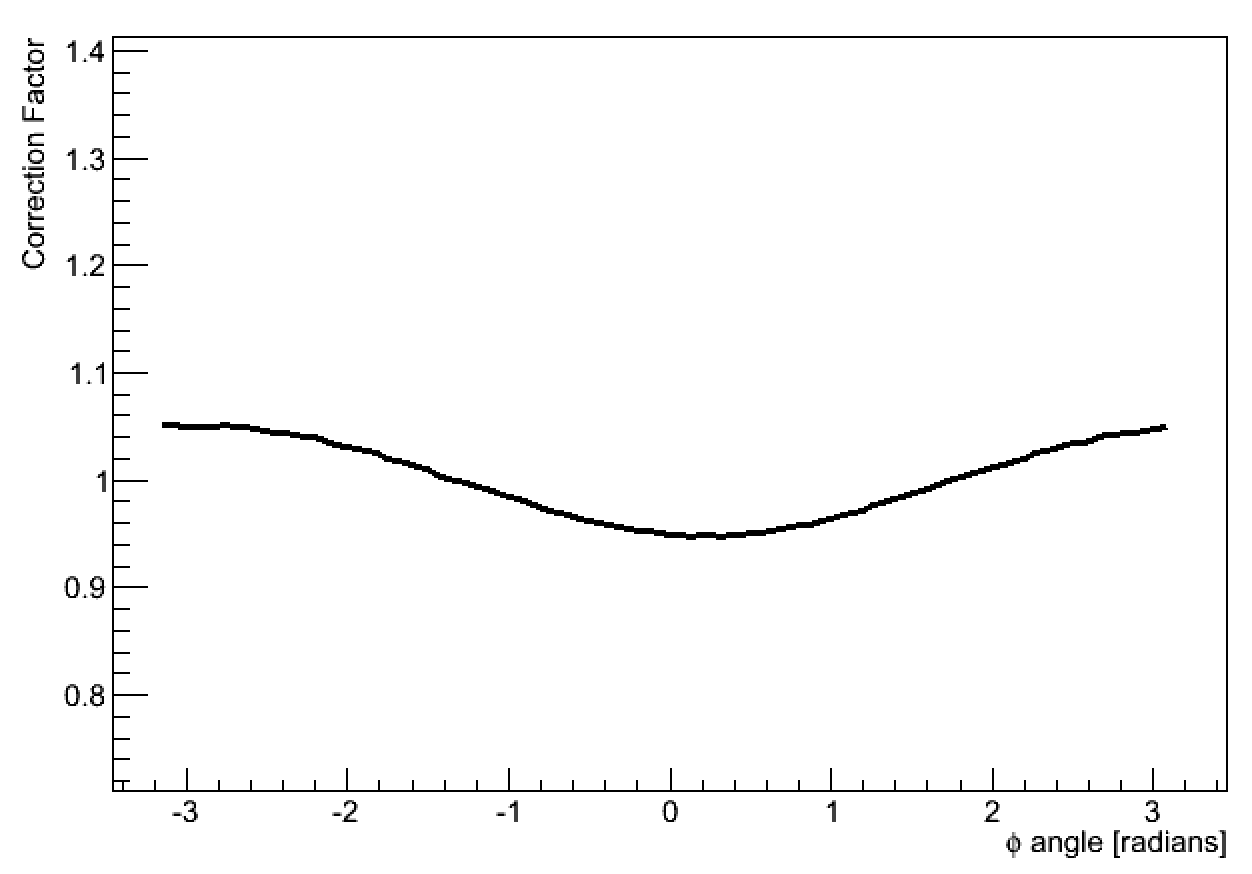
\includegraphics[width=0.47\linewidth]{figs/analytic_correction.png}
\caption{The modification of the $\eta$ acceptance as a function of $\phi$ for the FVTX first layer (left) and the calculated correction factor from this modification (right).}
\label{fig:analytic_corr}
\end{figure}

\subsection{FVTX Inverse Phi Weighting}
\label{sec:FVTX_inv_phi_weight}
Another way to determine the weight factor is to use a data driven method of measuring the extent to which each $\phi$ region in a detector has systematically more or less particles. Then an inverse weighting based on this measurement is applied to the $\phi$ regions to correct the $\phi$ distribution of the detector to uniformity.

For the FVTX implementation of this, first the rotation and offset correction are applied. Then, the weight factor is determined by plotting all hits in a cylindrical disk detector vs $\phi$, normalizing this distribution to one, and then inverting it. Applying this weight factor to the data will produce uniform hit distributions in $\phi$ in each of the detectors to which it is applied. This will, in turn, make the event plane distribution more uniform when measured in those detectors, thus correcting for the effect. The added benefit of using this method is that it also corrects for hot and cold $\phi$ regions in the detector. In order to get rid of significant hot or cold $\phi$ regions, $\phi$ regions with weight factors greater than 1.5 or less than 0.5 are set to 0.0. This correction is done for each FVTX layer, in z-vertex bins, and on a run-by-run basis. The multiplicative weight function $F(\phi,z_{\rm vertex})$ for the FVTX disks is defined as 
\begin{equation}
F(\phi,z_{\rm vertex},layer) = \frac{\left<N_{\rm cluster}(z_{\rm vertex},layer)\right>}{N_{\rm cluster}(\phi,z_{\rm vertex},layer)},
\end{equation}
where $N_{\rm cluster}(\phi,z_{\rm vertex},layer)$ is the number of FVTX clusters as a function of $\phi$, $z_{\rm vertex}$, and FVTX layer and $\left<N_{\rm cluster}(z_{\rm vertex},layer)\right>$ is the $\phi$ average of the number of clusters. The weighting can be seen in Figure~\ref{fig:fvtx_weighting}. A comparison between the FVTX weighting and the analytic correction is shown in Figure~\ref{fig:analytic_comparison}. The good agreement indicates the validity of the weighting.

\begin{figure}[!ht]
\centering
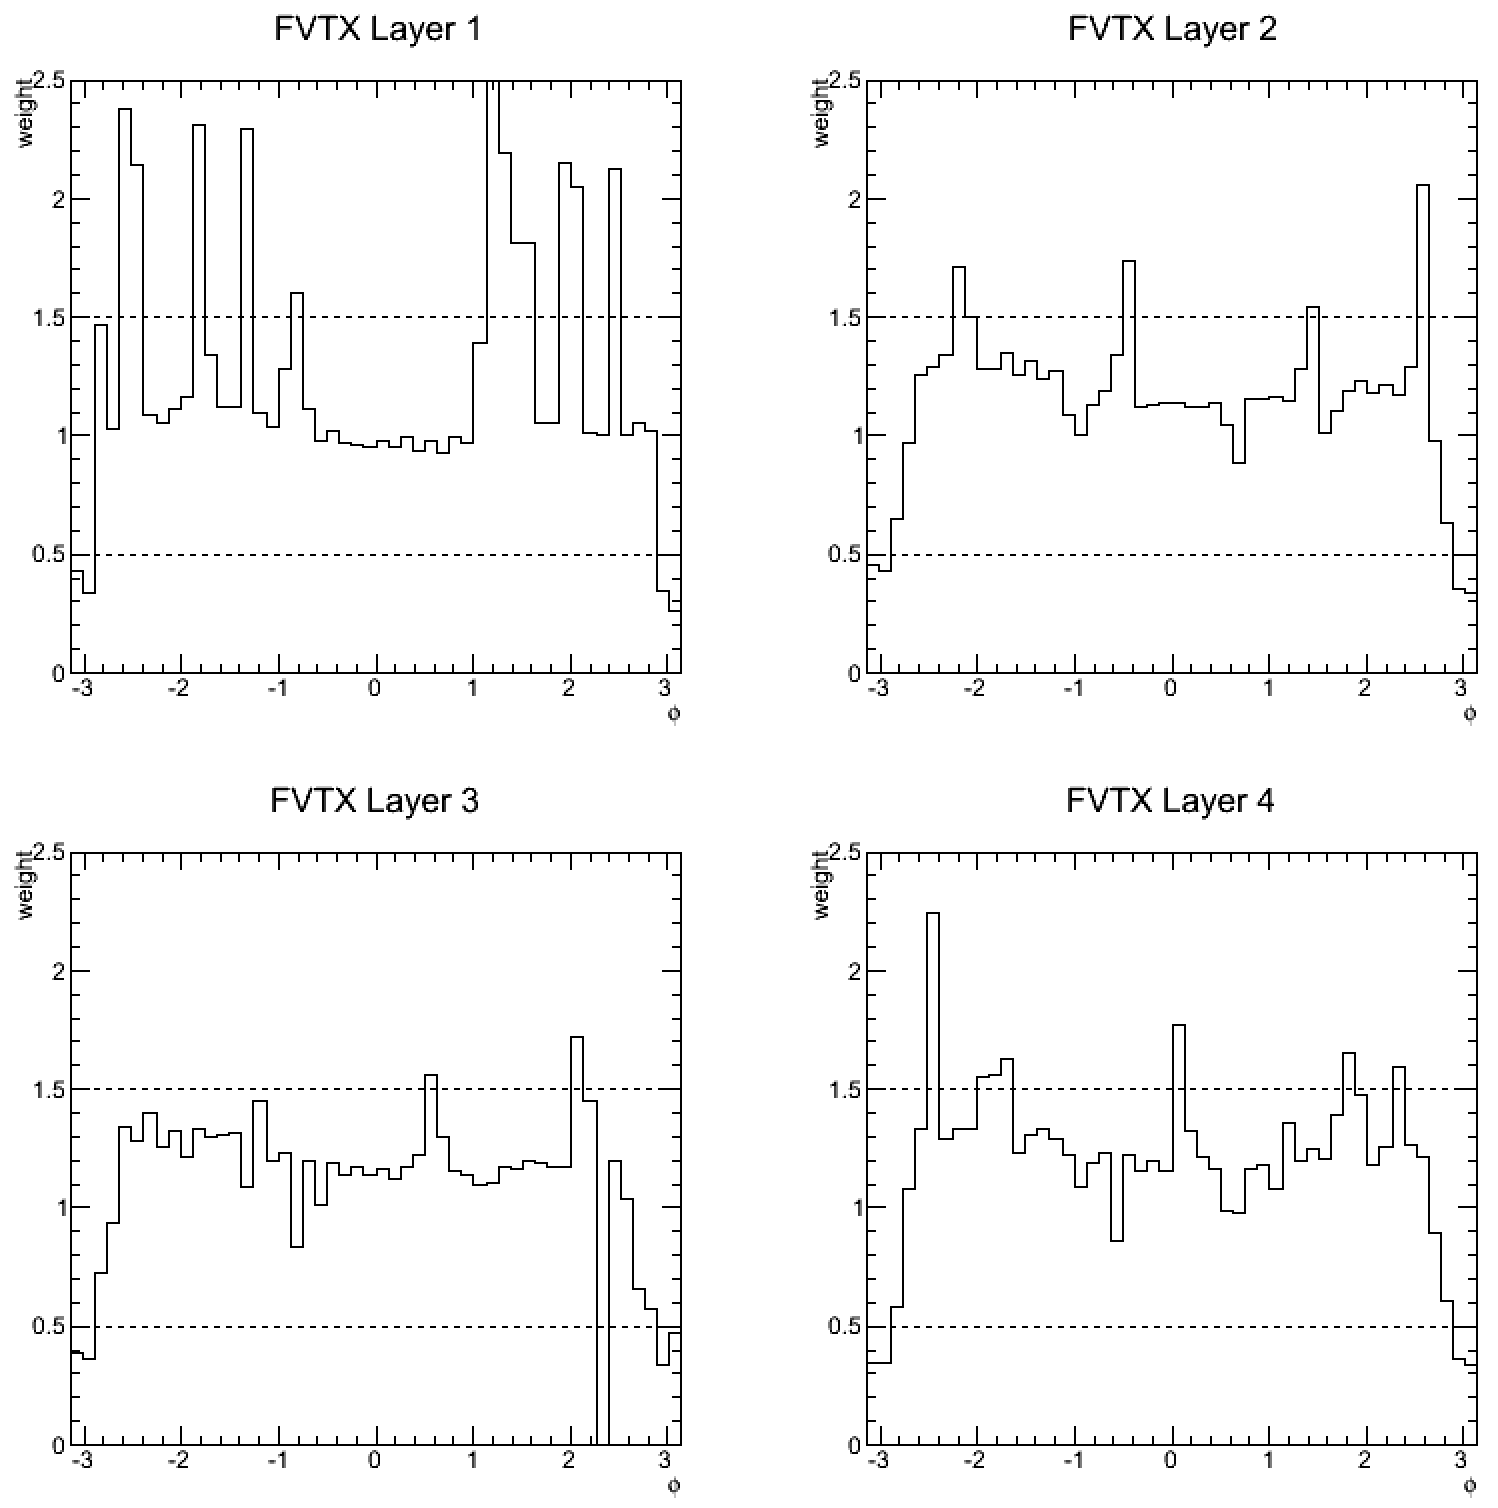
\includegraphics[width=0.75\linewidth]{figs/fvtx_weighting.png}
\caption{These four panels show the FVTX $\phi$ dependent cluster weighting when calculating the FVTX event plane for each layer separately for events when a collision vertex in $z$ is around 0. There are some $\phi$ regions where weight factor is outside of the dotted line bounds. This indicates that either there was a severe deficit or excess of clusters measured in the region. Later, we will examine the effect of keeping these regions or cutting them out on the $v_2$ measurement.}
\label{fig:fvtx_weighting}
\end{figure}
\begin{figure}[!ht]
\centering
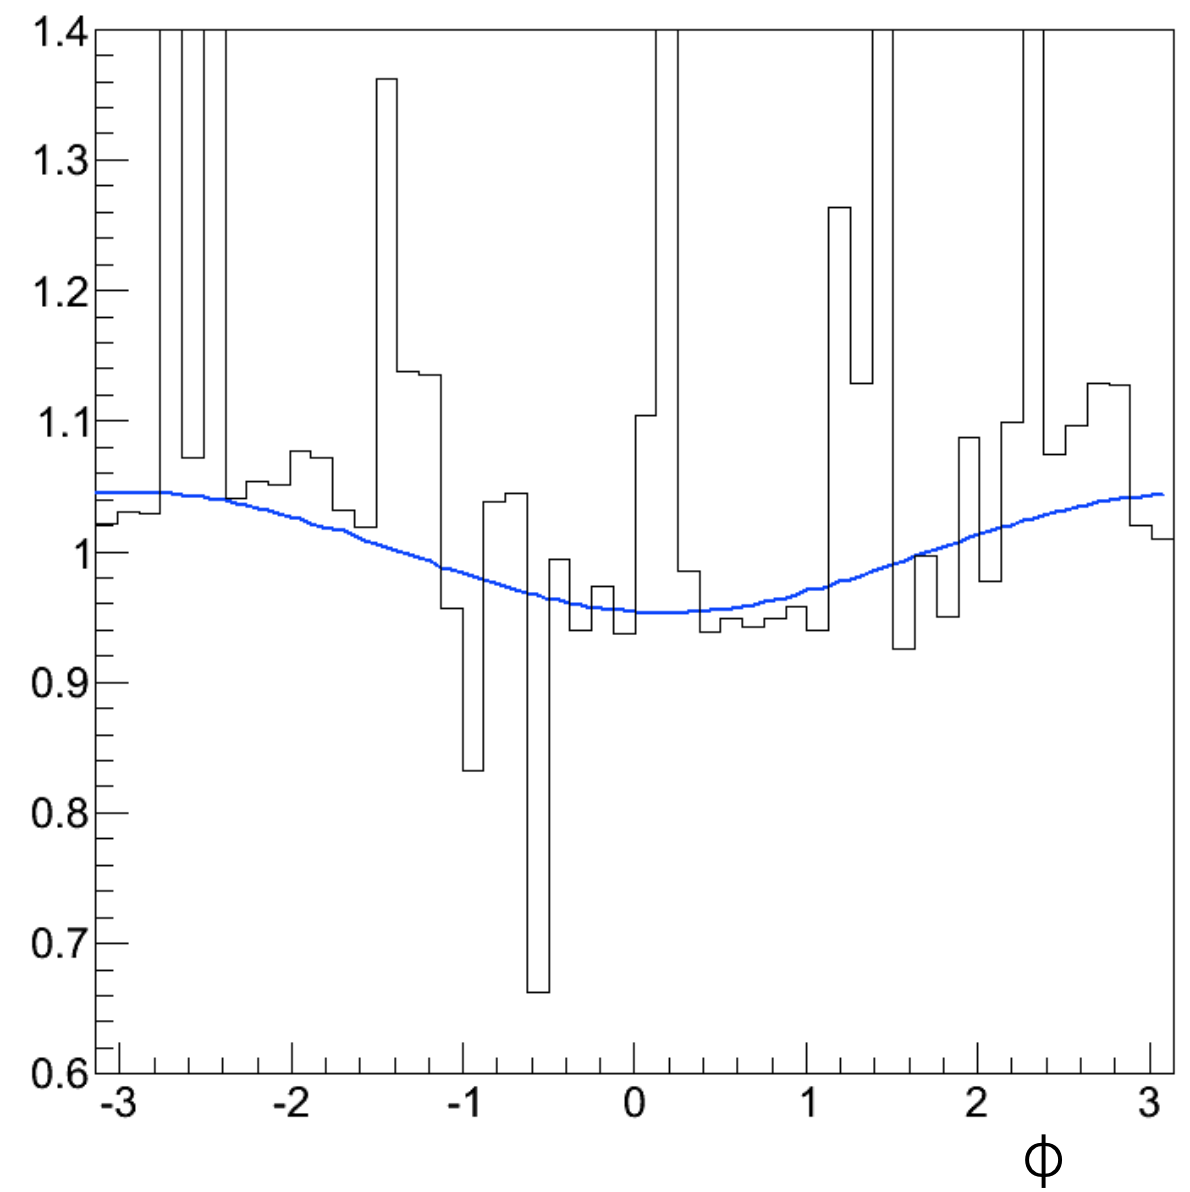
\includegraphics[width=0.5\linewidth]{figs/comparison_of_weights.png}
\caption{The black is the FVTX weighting and the blue is the analytic weighting. They have good agreement.}
\label{fig:analytic_comparison}
\end{figure}

\subsection{BBC Charge Weighting}
\label{sec:bbc_charge_weight}
For the BBC, we used another data driven method to correct for the non-uniform particle distribution. Using the distribution of particles in the BBC from the 2015 \pp $\sqrt{s}$ = 200 dataset as a baseline, we applied an inverse weighting much like the method described in the previous section. In the \pp dataset, there was no issue with beams colliding at an angle and the average charge across all 64 PMTs in the BBCS is uniform. In this method, the multiplicative weight function $F(PMT,z_{\rm vertex})$ for the BBCS is defined as:
\begin{equation}
F(PMT,z_{\rm vertex}) = \frac{\left<N^{\pp}_{Charge}(z_{\rm vertex})\right>}{\left<N^{\pau}_{Charge}(PMT,z_{\rm vertex})\right>},
\end{equation}
where $\langle N^{\pp,\pau}_{Charge}(PMT,z_{\rm vertex})\rangle$ is the event averaged charge as a function of PMT and $z_{\rm vertex}$ for the \pp and \pau datasets, respectively. 
This weight function is shown in Figure~\ref{fig:bbc_weight_function} and is applied directly to the event plane calculation using Equations \ref{eqn:bbc_ep_eqns} and  \ref{eqn:modified_weight}. 
Although the weight function could be defined as a function of $\phi$ like in the FVTX case, the positions of the PMTs in the BBC are fixed and it is more direct to take the ratio between PMTs.

\begin{figure}[!ht]
\begin{center}
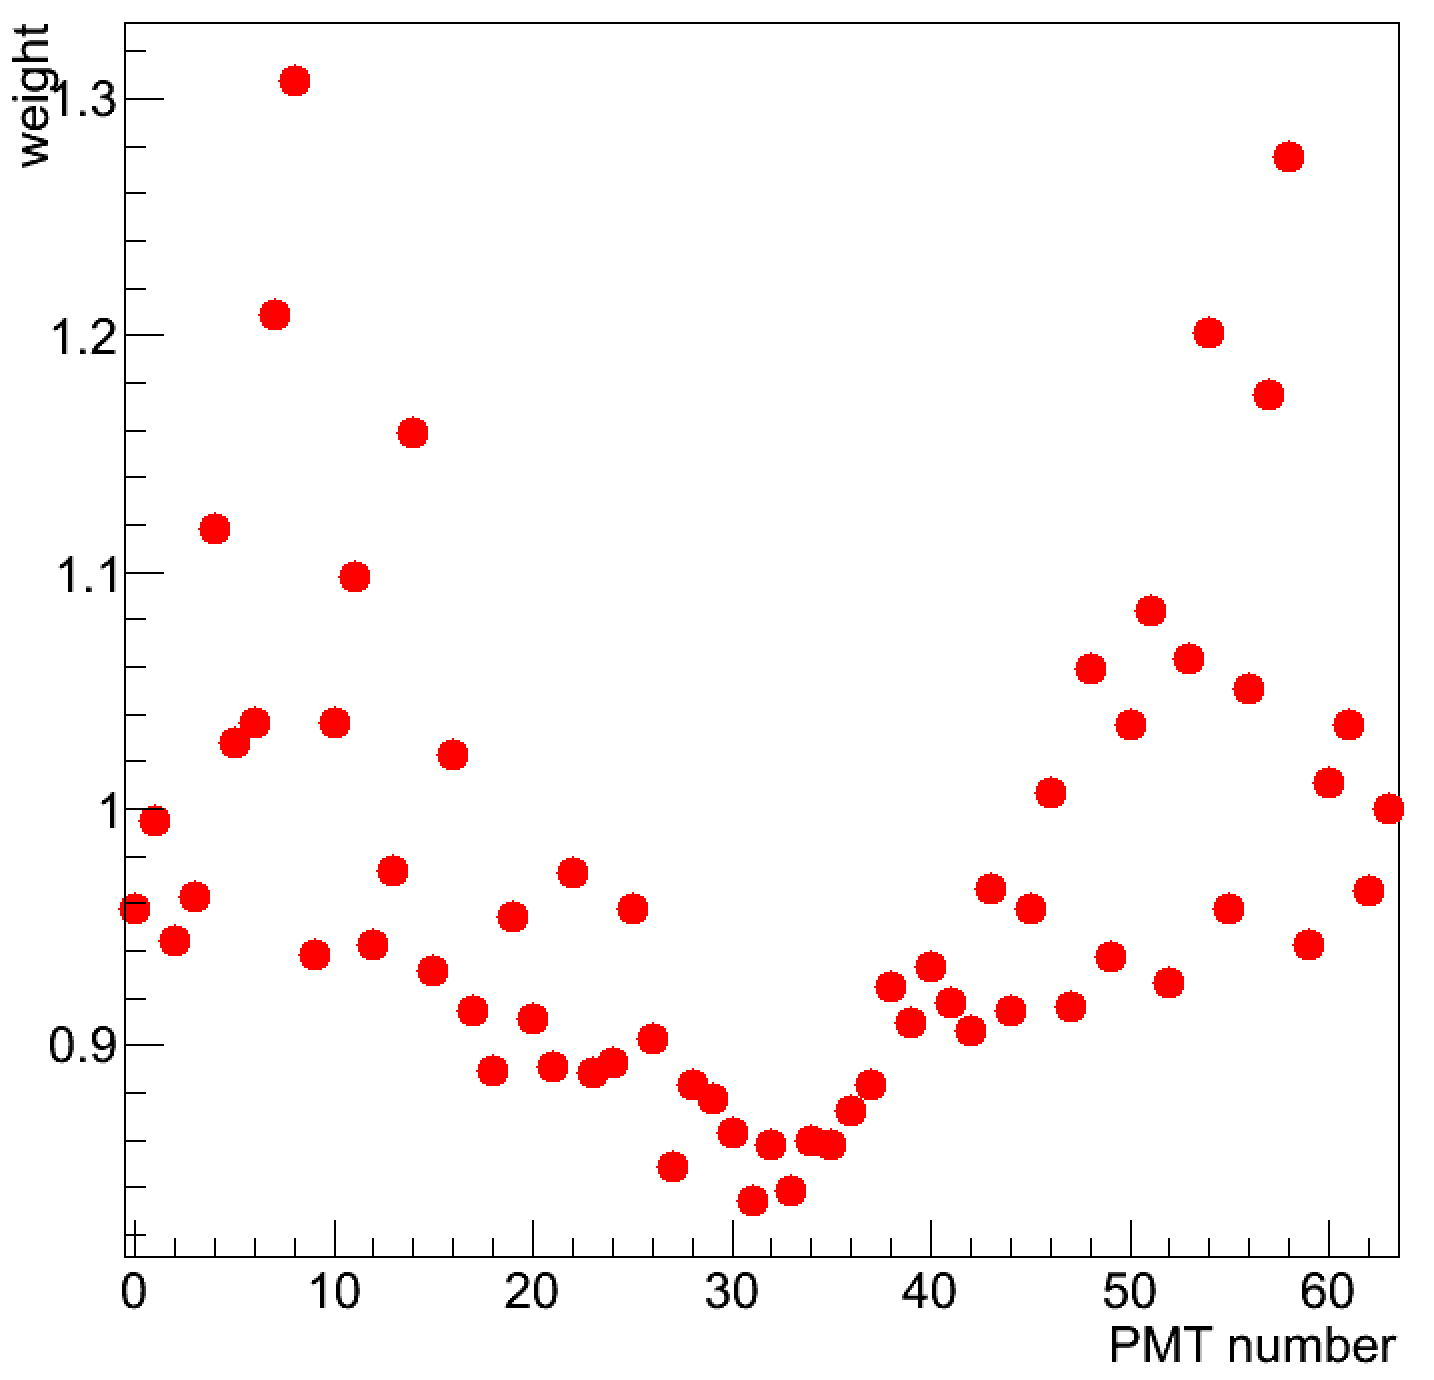
\includegraphics[width=0.5\linewidth]{figs/pmt_ratio_weight.png}
\caption{Shown here is BBC the multiplicative weight factor $F$ used when calculating the modified event plane for events where the collision vertex in z is around 0. The $y$-axis is the weight factor and the x-axis is the PMT number for the BBCS (there are 64 total in the BBCS). }
\label{fig:bbc_weight_function}
\end{center}
\end{figure}

One effect of using this weighting method is that it will make the distribution of particles in the BBC in $\phi$ and $\eta $ uniform. This can be illustrated by looking at Figure~\ref{fig:bbc_pmt_phi_pp_pau}. It is apparent that the \pp average charge is much more uniform than the \pau average charge as a function of $\phi$ and ring. After applying the \pp/\pau ratio weighting, which is essentially dividing the left plot by the right plot in Figure~\ref{fig:bbc_pmt_phi_pp_pau}, the PMT charges in ring 1 for the \pau dataset will be deweighted so that their corrected average charge will be uniform in $\phi$, and in agreement with the average charge for the other rings. If all the BBC rings have the same average charge, this means that the average charge as a function of $\eta$ for the BBC will be approximately uniform. This is one reason why this method (\pp/\pau ratio weighting) is preferred for the BBC, because the variations in the average charge between the rings are normalized. One could apply the FVTX method of inverse $\phi$ weighting by inverting the right plot of Figure~\ref{fig:bbc_pmt_phi_pp_pau} to find the weight function. However, although using only the \pau dataset would normalize the average charge as a function of $\phi$, it would not normalize the charge as a function of $\eta$. Both methods are applied to the data and shown in the next section.

\begin{figure}[!ht]
\begin{center}
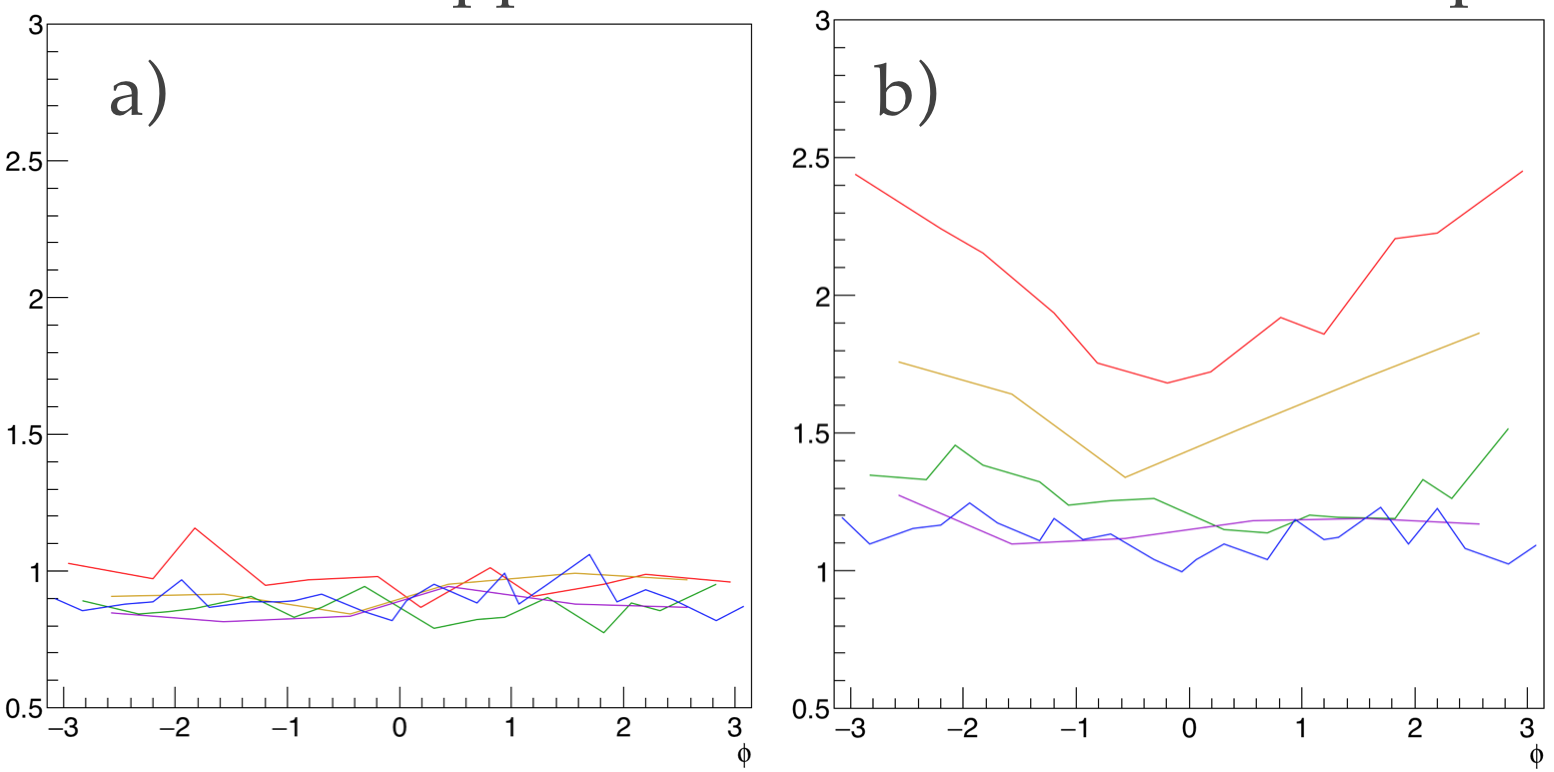
\includegraphics[width=0.75\linewidth]{figs/pp_pau_bbc_comparison.png}
\caption{These plots depict the average PMT charge per event versus $\phi$ in the a) the \pp $\sqrt{s}$ = 200 GeV and b) \pau \sqsn = 200 GeV. The PMTs are separated by color, which corresponds to the rings of approximate common radius as shown in Figure~\ref{fig:bbc_rings}. The left plot shows near uniformity as a function of $\phi$ and ring. However, the right plot shows a significant deviation from uniformity especially for the innermost rings (rings 1 and 2). In addition to the $\phi$ variation for the right plot, the innermost rings have the largest average charge when compared to the other rings. This is in part due to the fact the innermost rings cover the a slightly larger $\eta$ range. However, the innermost rings in the left plot also cover the largest $\eta$ range and do not exhibit this separation in rings. }
\label{fig:bbc_pmt_phi_pp_pau}
\end{center}
\end{figure}

\subsection{Applying Weighting to v2}
The previously discussed corrections are applied when calculating the raw $\Psi_2^{\rm FVTXS}$ used in the $v_2$ measurement. Shown in Figure \ref{fig:fvtx_corr_summary} is the correction summary for the FVTXS $v_2$ measurement where $R_{v_2^{\rm FVTXS}}$ is the y-axis. The first column, which corresponds to $R_{v_2^{\rm FVTXS}}$ calculated using FVTXS layers 1, 2, and 4, with layer 3 being excluded, is explained shortly. The black, red, blue, and green points correspond to no weighting, analytic weighting, inverse $\phi$ weighting, and inverse $\phi$ weighting with cuts, respectively. Compared to the $R_{v_2^{\rm FVTXS}}$ calculated with no weighting, $R_{v_2^{\rm FVTXS}}$ calculated with each of the corrections brings the ratio quantity much closer to 1.0, indicating the weighting techniques are working.  In order to better understand the effect of the corrections, $R_{v_2^{\rm FVTXS}}$ is measured separately with each FVTXS layer. The rationale for this exclusion is due to FVTXS layer 3's unusual behavior in relation to the other FVTXS layers. As we go from layer 1 to layer 4, the $R_{v_2^{\rm FVTXS}}$ generally is trending downward except for layer 3. Although the reason for this was never definitively determined, it is likely there is some issue with the layer data due to electronic or detector problems. Thus, the measurement of $v_2^{\rm FVTXS}$ is calculated without any clusters in the third layer.

\begin{figure}[!h]
\begin{center}
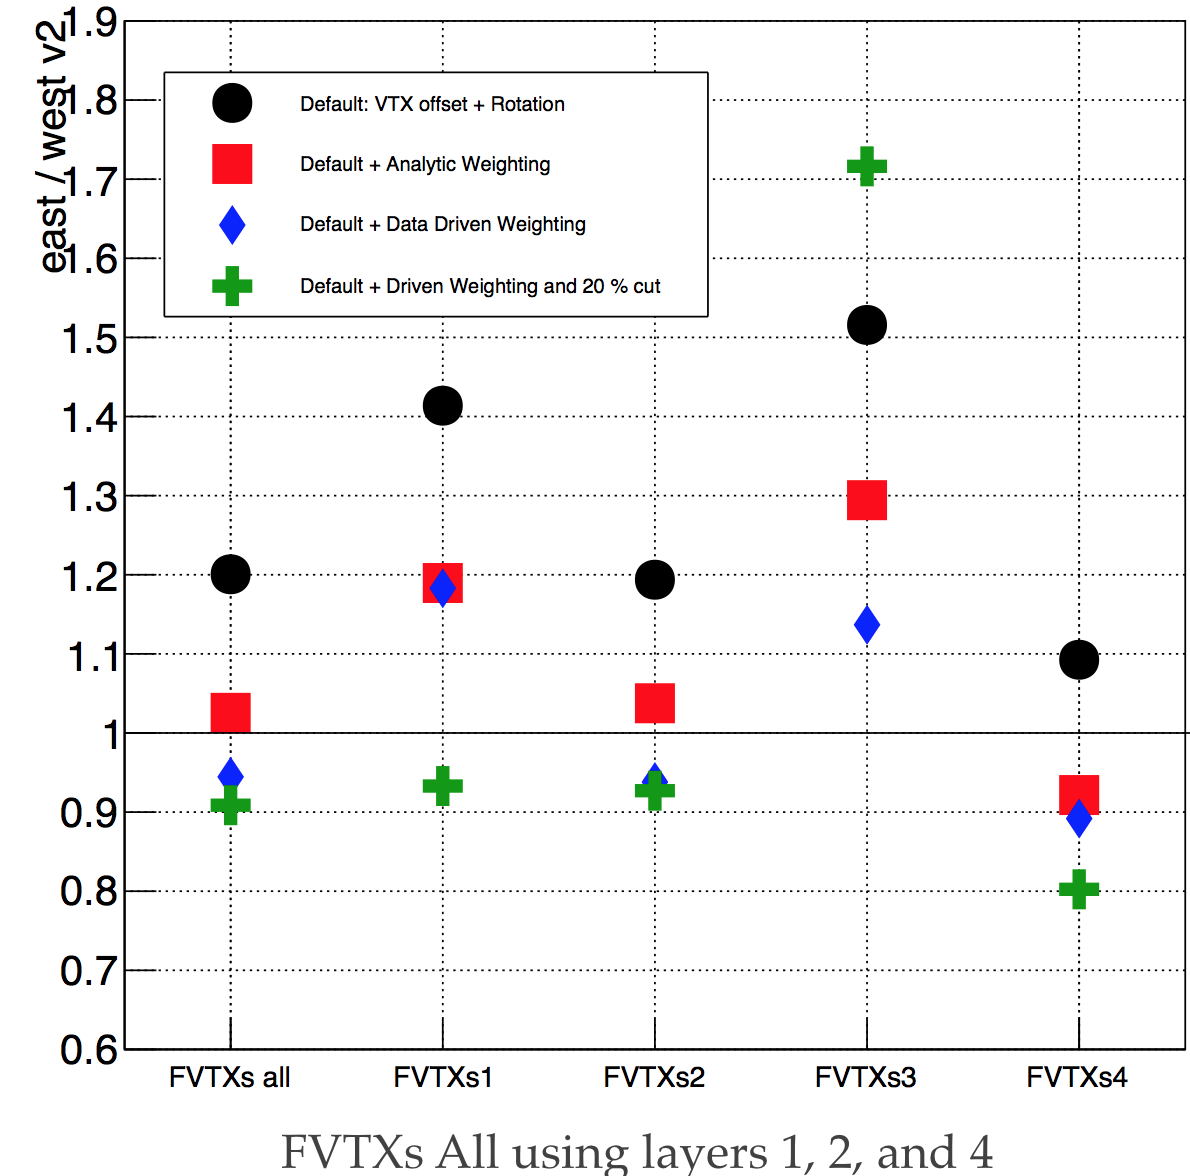
\includegraphics[width=0.5\linewidth]{figs/fvtx_correction_summary.png}
\caption{Plotted is the FVTXS correction summary where the y-axis is the east/west $v_2$ ratio and the x-axis is the different subset of clusters used to calculate the $v_2$. The black markers correspond to the default corrections. The red boxes correspond to the corrections with the analytic weighting shown in Figure~\ref{fig:analytic_corr}. The blue diamonds are the FVTX inverse $\phi$ weighting as shown is section \ref{sec:FVTX_inv_phi_weight}. Finally, the green crosses correspond to the same as the blue diamonds except an additional hot-cold filter of 20\% was applied. The first column is using all the FVTXS layers except for the 3rd layer (explained in the text). So the first columns should be approximately the average of columns 2, 3, and 5. Columns 2 through 5 show the ratio calculated from clusters only in that layer.}
\label{fig:fvtx_corr_summary}
\end{center}
\end{figure}

Similarly, Figure \ref{fig:bbc_corr_summary} is the correction summary for the BBCS $v_2$ measurement where $R_{v_2^{\rm BBCS}}$ is the y-axis. The first column corresponds to $R_{v_2^{\rm BBCS}}$ calculated using all five BBCS rings. Compared to the $R_{v_2^{\rm BBCS}}$ when calculated with no weighting, $R_{v_2^{\rm BBCS}}$ when calculated with the data driven and \pp/\pau ratio weighting is modestly closer to 1.0. By looking at $R_{v_2^{\rm BBCS}}$ calculated with PMTs in individual BBCS rings for the weighted points, $R_{v_2^{\rm BBCS}}$ is generally trending downward as a function of ring number. Applying the weighting corrections to $R_{v_2^{\rm BBCS}}$ calculated by ring 1, the innermost ring, over-corrects $R_{v_2^{\rm BBCS}}$. This may be explained by the fact that ring 1 covers the largest $\eta$ acceptance range, causing the correction to be inconsistent. The reason ring 1 is not excluded from the inclusive $v_2$ calculation, like the FVTXS layer 3 is excluded, is because there is no reasonable justification to exclude it other than its over-corrected $R_{v_2^{\rm BBCS}}$ values. While FVTXS layer 3 breaks the trend of $R_{v_2^{\rm FVTXS}}$ decreasing, BBCS ring 1 follows the $R_{v_2^{\rm BBCS}}$ ring trend. See appendix \ref{sec:appendix} for the full $v_2(\pt)$ measurements for each event plane detector, each correction, and each layer or ring.

\begin{figure}[!h]
\begin{center}
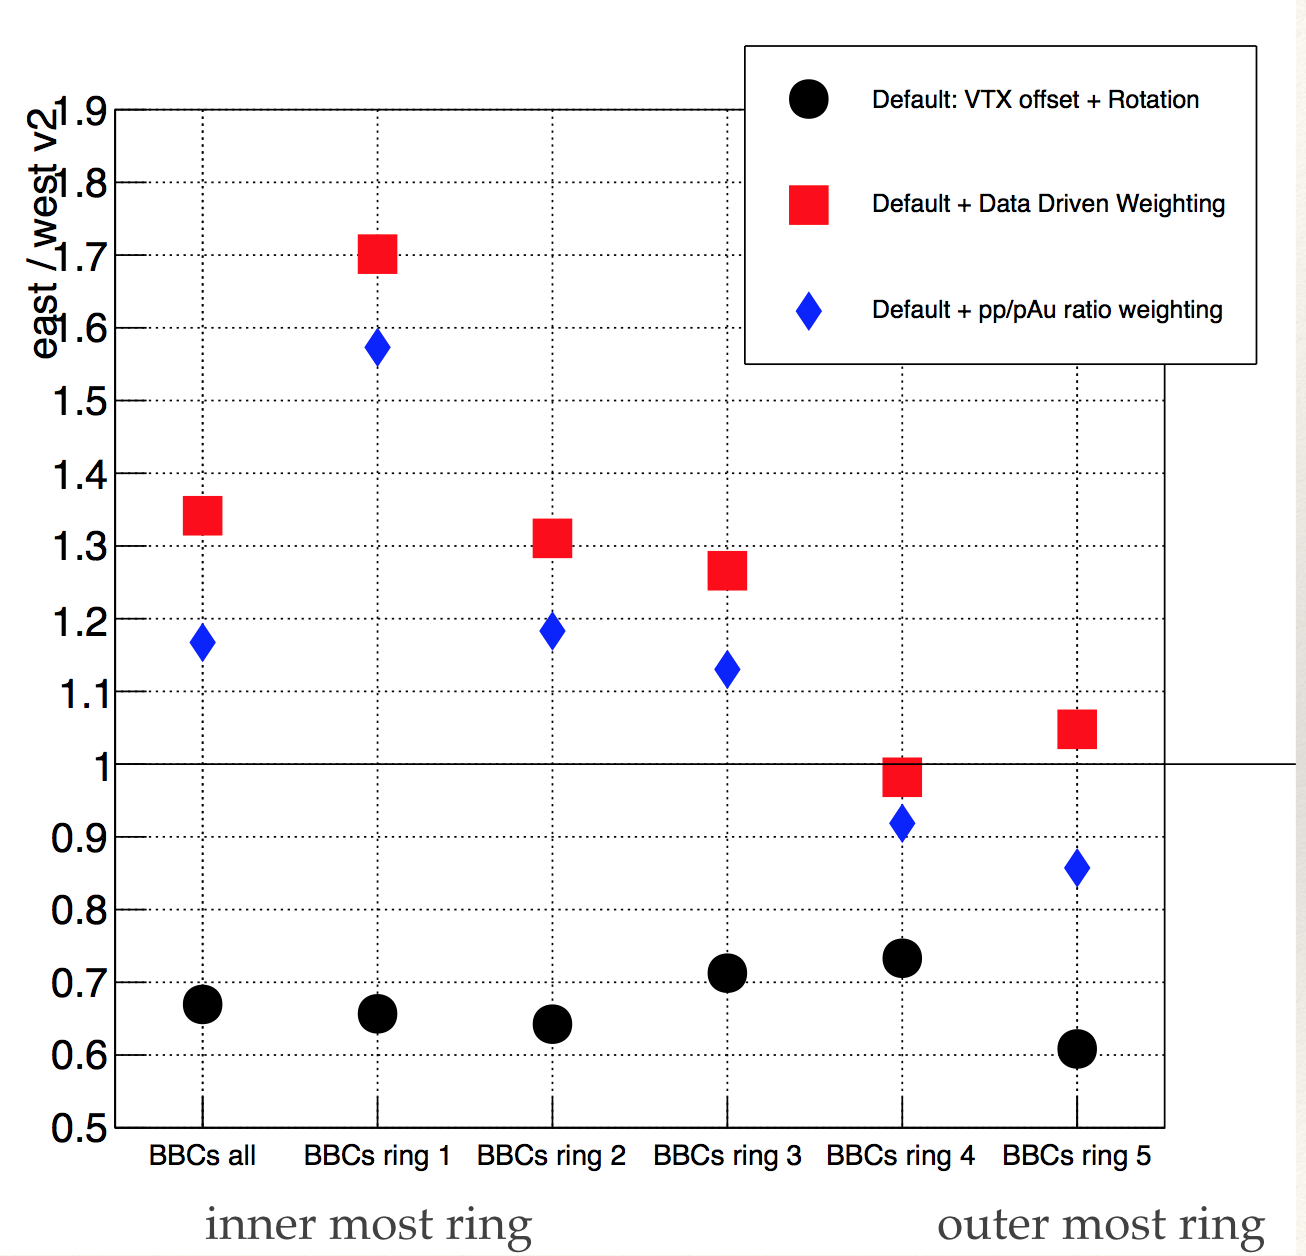
\includegraphics[width=0.5\linewidth]{figs/bbc_correction_summary.png}
\caption{Plotted is the BBC correction summary where the y-axis is the east/west $v_2$ ratio and the $x$-axis is the different subset of PMTs used to calculate the $v_2$. The black markers correspond to the default corrections. The red boxes correspond to the corrections with the analytic weighting shown in Figure~\ref{fig:analytic_corr}. Finally, the blue diamonds correspond to the BBC inverse $\phi$ charge weighting as shown in Section \ref{sec:bbc_charge_weight}. The first column is the quantity calculated from all PMTs. Columns 2 through 6 are using PMTs from certain rings as defined in Figure~\ref{fig:bbc_rings}. Ring 1 is the hardest to correct. The first column should approximately be the average of all the other columns.}
\label{fig:bbc_corr_summary}
\end{center}
\end{figure}

Figure~\ref{fig:fvtx_corrected_best} shows the $v_2(p_T)$ with the inverse $\phi$ weighting and 20\% cut from Figure \ref{fig:fvtx_corr_summary}. This figure also shows $v_2(p_T)$ with the pp/pAu ratio weighting from Figure~\ref{fig:bbc_corr_summary}. Although the east and west $v_2^{\rm BBCS}$ measurements do not collapse together like the east and west $v_2^{\rm FVTXS}$ measurements, the result is good enough to be incorporated in our systematics uncertainties. Due to the fact that $R_{v_2^{\rm FVTXS}}$ is corrected to within $\pm10\%$ and the fact that $v_2^{\rm FVTXS}(p_T)$ has a smaller statistical uncertainty, the primary $v_2(p_T)$ measurement is done using the FVTXS.

\begin{figure}[!h]
\begin{center}
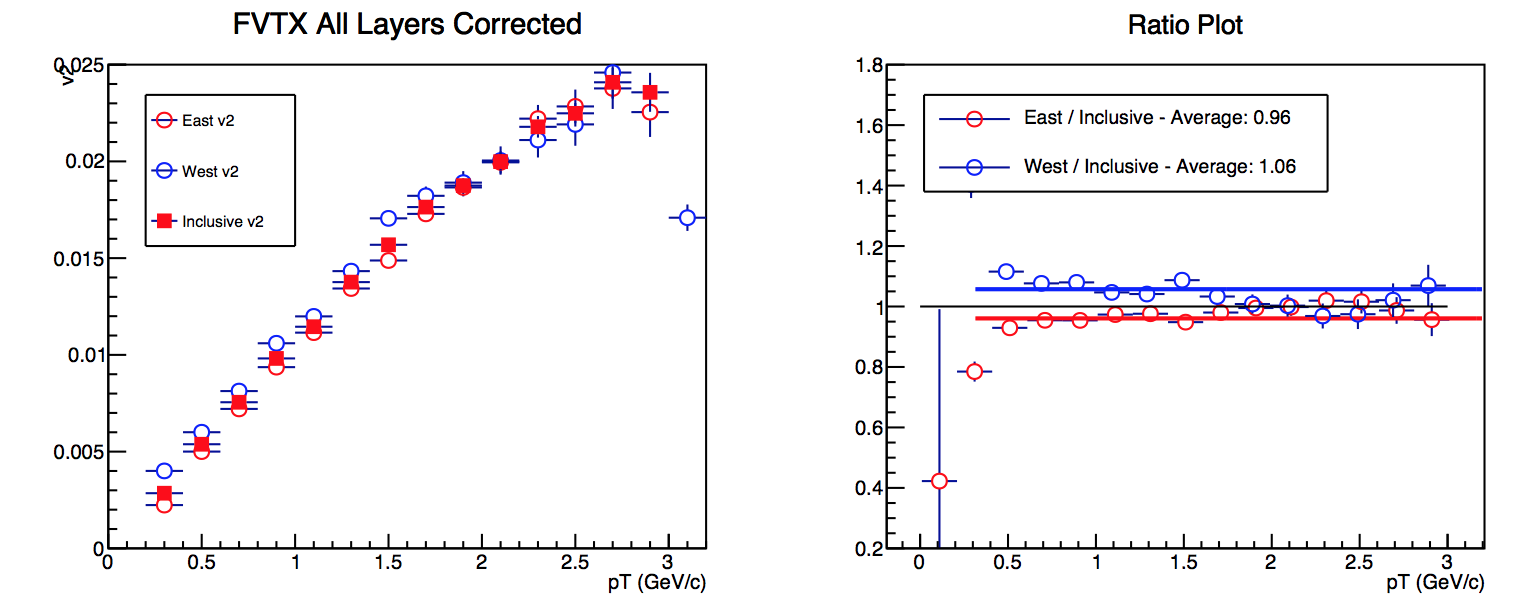
\includegraphics[width=0.75\linewidth]{figs/fvtx_corrected.png}
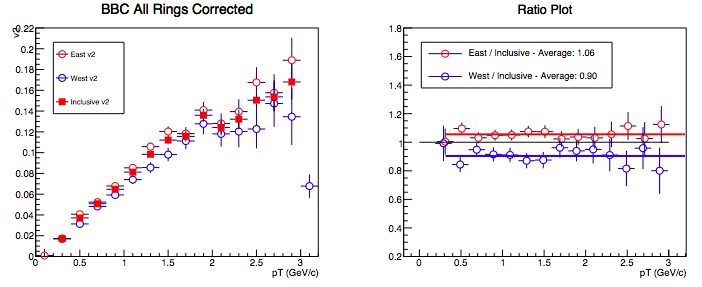
\includegraphics[width=0.75\linewidth]{figs/bbc_pp_correction.png}
\caption{ FVTXS $v_2$ event plane measurement corrected with inverse $\phi$ weighting and 20 $\%$ cut with FVTXS layer 3 is excluded (top) and BBCS $v_2$ event plane measurement corrected with \pp/\pau ratio weighting (bottom).}
\label{fig:fvtx_corrected_best}
\end{center}
\end{figure}

In order to estimate the contribution of this systematic uncertainty, we assume the true $v_2$ value is absolutely bounded between the separate east and west measurements and we assume that the probability distribution for $v_2$ is uniformly distributed between the upper and lower bounds. Thus, we calculate the point-by-point absolute value of $v_2^{\textrm{east}}$ minus the $v_2^{\textrm{west}}$ divided by $\sqrt{12}$, which is the RMS width of an uniform distribution. By using the best corrected BBCS $v_2$ measurement in this calculation, we assign a value of $5\%$ for this systematic uncertainty.

%\clearpage
%\begin{figure}[!h]
%\begin{center}
%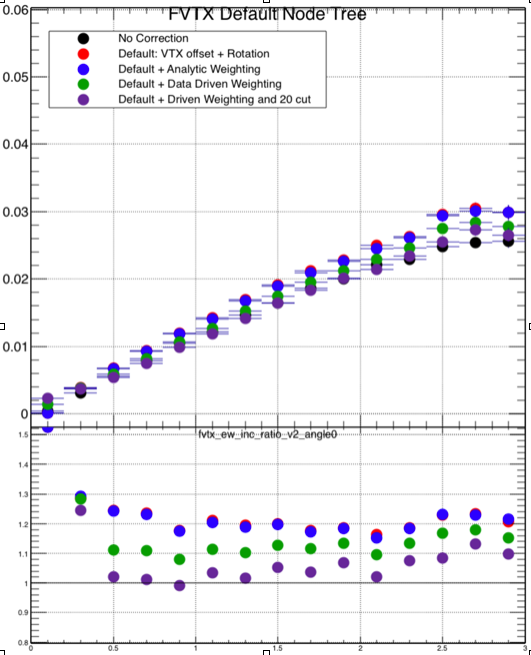
\includegraphics[width=0.5\linewidth]{figs/fvtx_incl_v2_comparison_corrections.png}
%\caption{}
%\end{center}
%\end{figure}

\section{Other Sources of Systematic Uncertainty}
In this section, other sources of systematic uncertainty are described and the sum of the systematic uncertainties are shown.
\subsection{Effect of Event Pile-Up}
Pile-up events occur when there are two or more collisions within the same bunch crossing. Pile-up events are an issue for this analysis because they:
\begin{enumerate}
\item are erroneously included into the 0-5\% centrality selection due to two low multiplicity collisions looking like a high multiplicity collision,
\item and reduce the value of $v_2$ because the event plane angle from one collision will be different than the event plane angle in the other collision, such that correlations calculated by using particles produced from the two collisions are random and will dilute the real correlations, thereby reducing the flow signal.
\end{enumerate}

In order to filter pile-up events we look at the distribution of BBC PMT timing values as seen in Figure~\ref{fig:pile_up_example}. A normal event is strongly peaked at 0 while a pile-up event has a broad distribution and may not be centered at 0. We developed an algorithm to efficiently filter pile-up events by analyzing the BBC PMT timing value distribution event by event. When the $v_2$ values are compared with and without the filter, a difference of 4\% is seen. 

Pile-up events occur at a rate of 8\% in 0-5\% central \pau collisions. Low-luminosity and high-luminosity subsets of the data were analyzed, and the systematic uncertainty was determined to be $^{+4\%}_{-0\%}$, since the $v_2$  was found to decrease in the events that contain a pile-up as expected.

\begin{figure}[!h]
\begin{center}
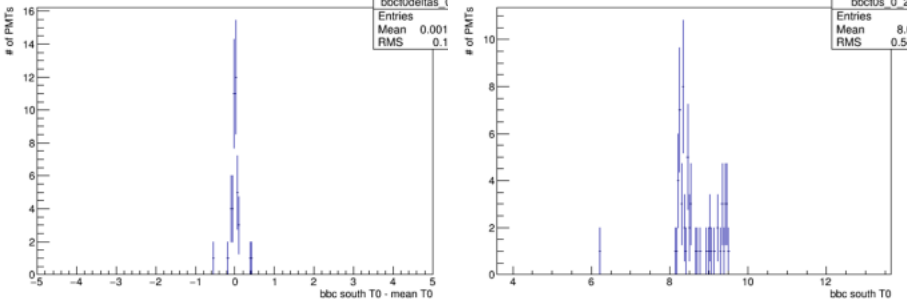
\includegraphics[width=0.8\linewidth]{figs/example_pile_up_event.png}
\caption{The distribution of BBC PMT timing values. The x-axis is the difference between the southern BBC PMT $t_0$ - the mean $t_0$ in the south. An example of a normal event (left) and an example pile-up event (right), are shown.}
\label{fig:pile_up_example}
\end{center}
\end{figure}

\subsection{Event Plane Detectors}
We expect that the value of $v_2$ should be consistent when measured in different detectors, after applying corrections. Any remaining difference of $v_2$ measured independently in the FVTXS and BBCS indicates a source of systematic uncertainty. The difference is calculated after applying corrections to beam alignment $v_2$, as shown in Figure \ref{fig:v2_fvtx_bbc_compare}. The right panel of the figure shows the average difference to be around 0.97. Thus, the systematic uncertainty estimated is $\pm$3\%.
\begin{figure}[!h]
\begin{center}
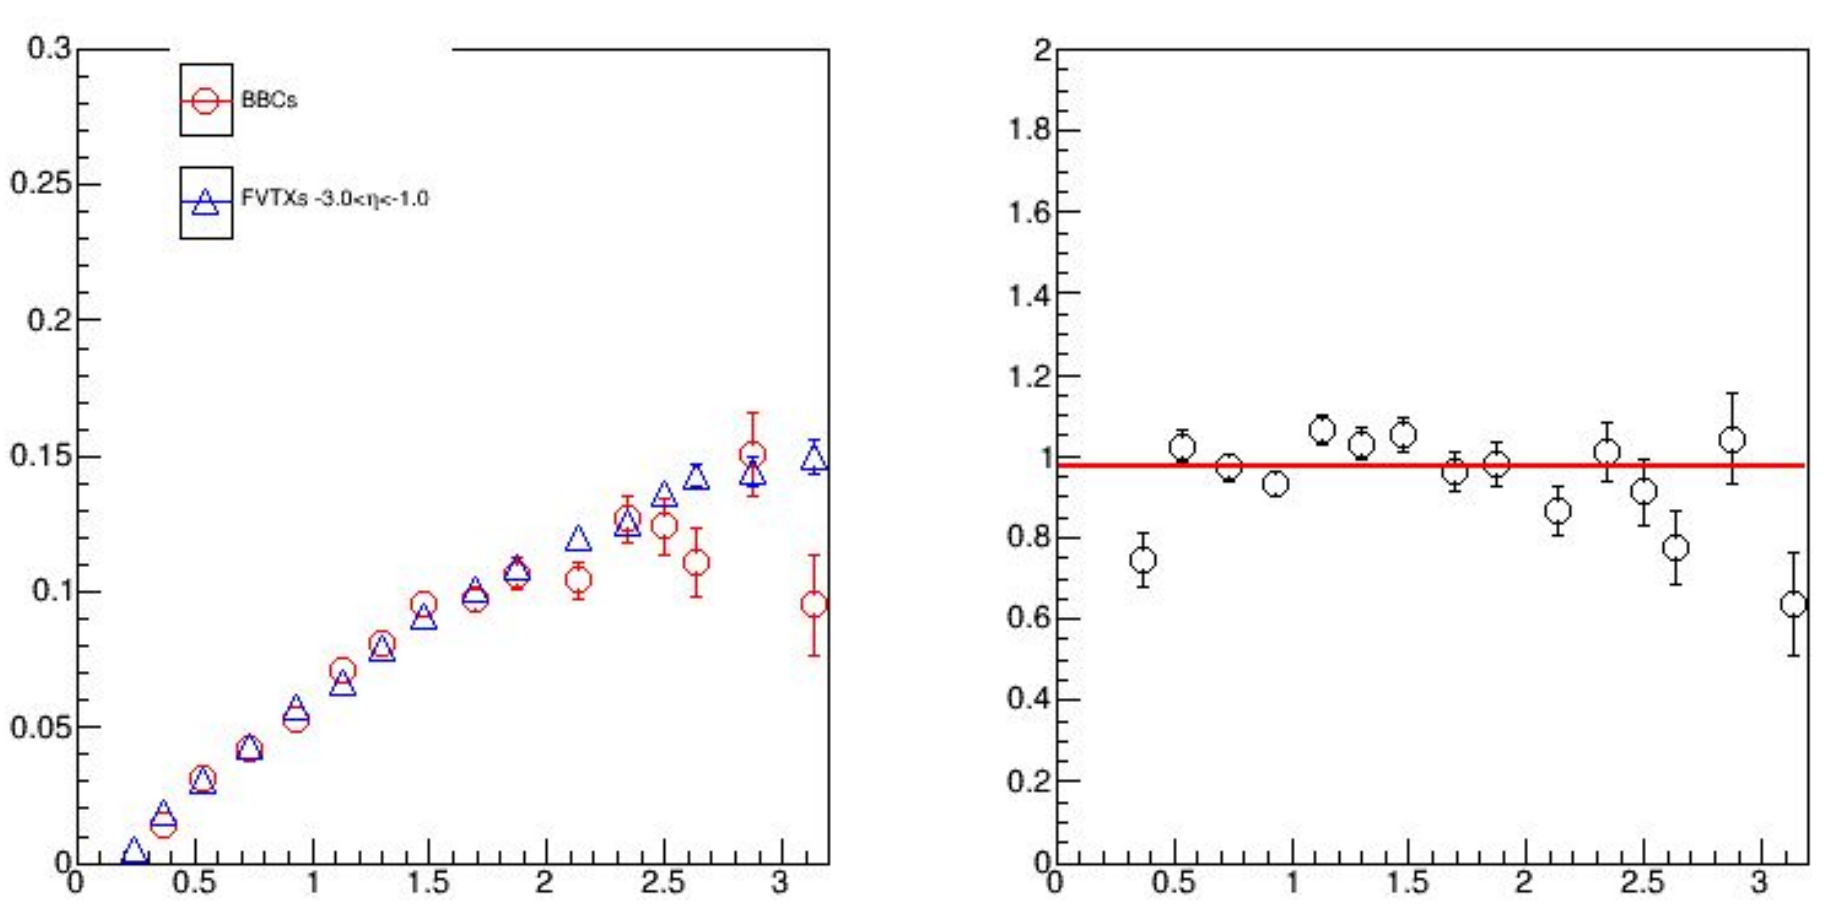
\includegraphics[width=0.6\linewidth]{figs/v2_fvtx_bbc_compare_w_correction.png}
\caption{$v_2(\pt)$ measured separately in the BBCS and the FVTXS after beam alignment corrections (left) and the ratio of $v_2^{\rm FVTXS}$ to $v_2^{\rm BBCS}$ (right). The red line is the average of the ratio across \pt.}
\label{fig:v2_fvtx_bbc_compare}
\end{center}
\end{figure}

\subsection{Track Background}
The set of tracks that are used in this analysis come from central arm tracks which are known to have a track background of 2.0\%. The track background from photonic conversions and weak decays, and mis-reconstructed tracks, which we estimate at 2\% relative to $v_2$ by varying the windows in the PC3 matching variables from 3$\sigma$ to 2$\sigma$.
\subsection{Effects of Non-Flow}
\label{sec:non_flow_intro}
%A short introduction on non-flow, may be placed in a different location later.
As discussed in Chapter 2, non-flow is a catch-all term used to categorize all types of angular correlations which do not arise from hydrodynamic flow and are not related to the initial collision geometry. Non-flow constitutes a significant background to our measurement. There are several known sources of non-flow:

\begin{enumerate}
\item hard scattering events producing dijets,
\item initial state correlations between target and projectile,
\item decay chains of exotic particles,
\item momentum conservation.
\end{enumerate}

Figure~\ref{fig:jet_corr_example} shows the characteristic two-particle correlations arising from non-flow associated with dijets. The near-side peak at (0,0) is from the cone of particles in a single jet all at a similar location in $\eta$ and $\phi$. The awayside ridge around $\phi$ = $\pi$ originates from particles pairs, where each particle belongs to a different jet. The two jets are completely back-to-back in $\Delta\phi$, but have a spread in $\Delta\eta$. This correlation function yields a substantial $c_2$ very similar to that from the hydrodynamic flow signal we are seeking. In order to minimize the contribution of dijet events, the standard flow analysis procedure is to select regions outside of the red dotted lines seen in Figure~\ref{fig:jet_corr_example} ($|\Delta\eta| > \eta_{min}$, where $\eta_{min}$ is usually on the order of 1.0 units of pseudorapidity).

\begin{figure}[!h]
\begin{center}
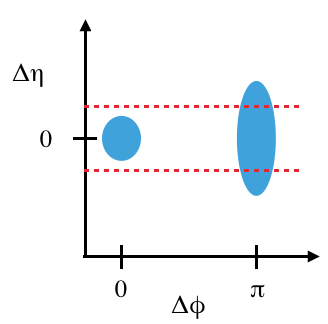
\includegraphics[width=0.5\linewidth]{figs/jet_corr_example.png}
\caption{2D profile of a correlation function in $\Delta\eta \Delta\phi$ space of a dijet event. The area bounded by red dotted lines represents the exclusion zone in $\Delta\eta$, such that the measurement is made only using data from outside of the exclusion zone to reduce non-flow contributions.}
\label{fig:jet_corr_example}
\end{center}
\end{figure}

In order to estimate the degree of presence of non-flow, we can measure the $c_2$ from \pp events which should be devoid of any hydrodynamic flow but should have many of the sources of non-flow present. In order to compare \pp with \pau, we must scale-up the \pp quantity by the dilution factor defined in Equation \ref{eq:dilute}. The scaled down reference $c_{2}$ is shown as blue squares in Fig.~\ref{fig:non_flow}, panel a). The ratio of $c_2$ in the scaled-down \pp reference to that in \pau is shown in panel b). 

From this ratio, as calculated in Equation \ref{eq:dilute}, it can be seen that the relative correlation strength in \pau from elementary processes is at most 23$\%$ at the highest $p_T$. Since this procedure constitutes an approximation to quantify the non-flow correlation strength, it is not subtracted from the total signal, instead it is treated as a source of systematic uncertainty. Even though the \pau and the \pp baseline data were collected in different years, such that potential changes in detector performance could affect our results, it was verified that using \pp data from various run periods has an effect of at most 3$\%$ on the calculated non-flow contribution. The non-flow correlations which enhance the $v_2$, whose contribution we estimate from Figure~\ref{fig:non_flow}, assigning a $p_T$-dependent asymmetric uncertainty with a maximum value of $^{+0}_{-23}\%$
\begin{equation}
c_{2}^{{\rm pAu \; elementary}}(p_{T}) \simeq c_{2}^{\pp}(p_{T})
\frac{\left( \sum Q^{{\rm \text{BBC-S}}} \right)_{\pp}}
{\left( \sum Q^{{\rm \text{BBC-S}}} \right)_{{\rm pAu}}}.
\label{eq:dilute}
\end{equation}

\begin{figure}[!h]
\begin{center}
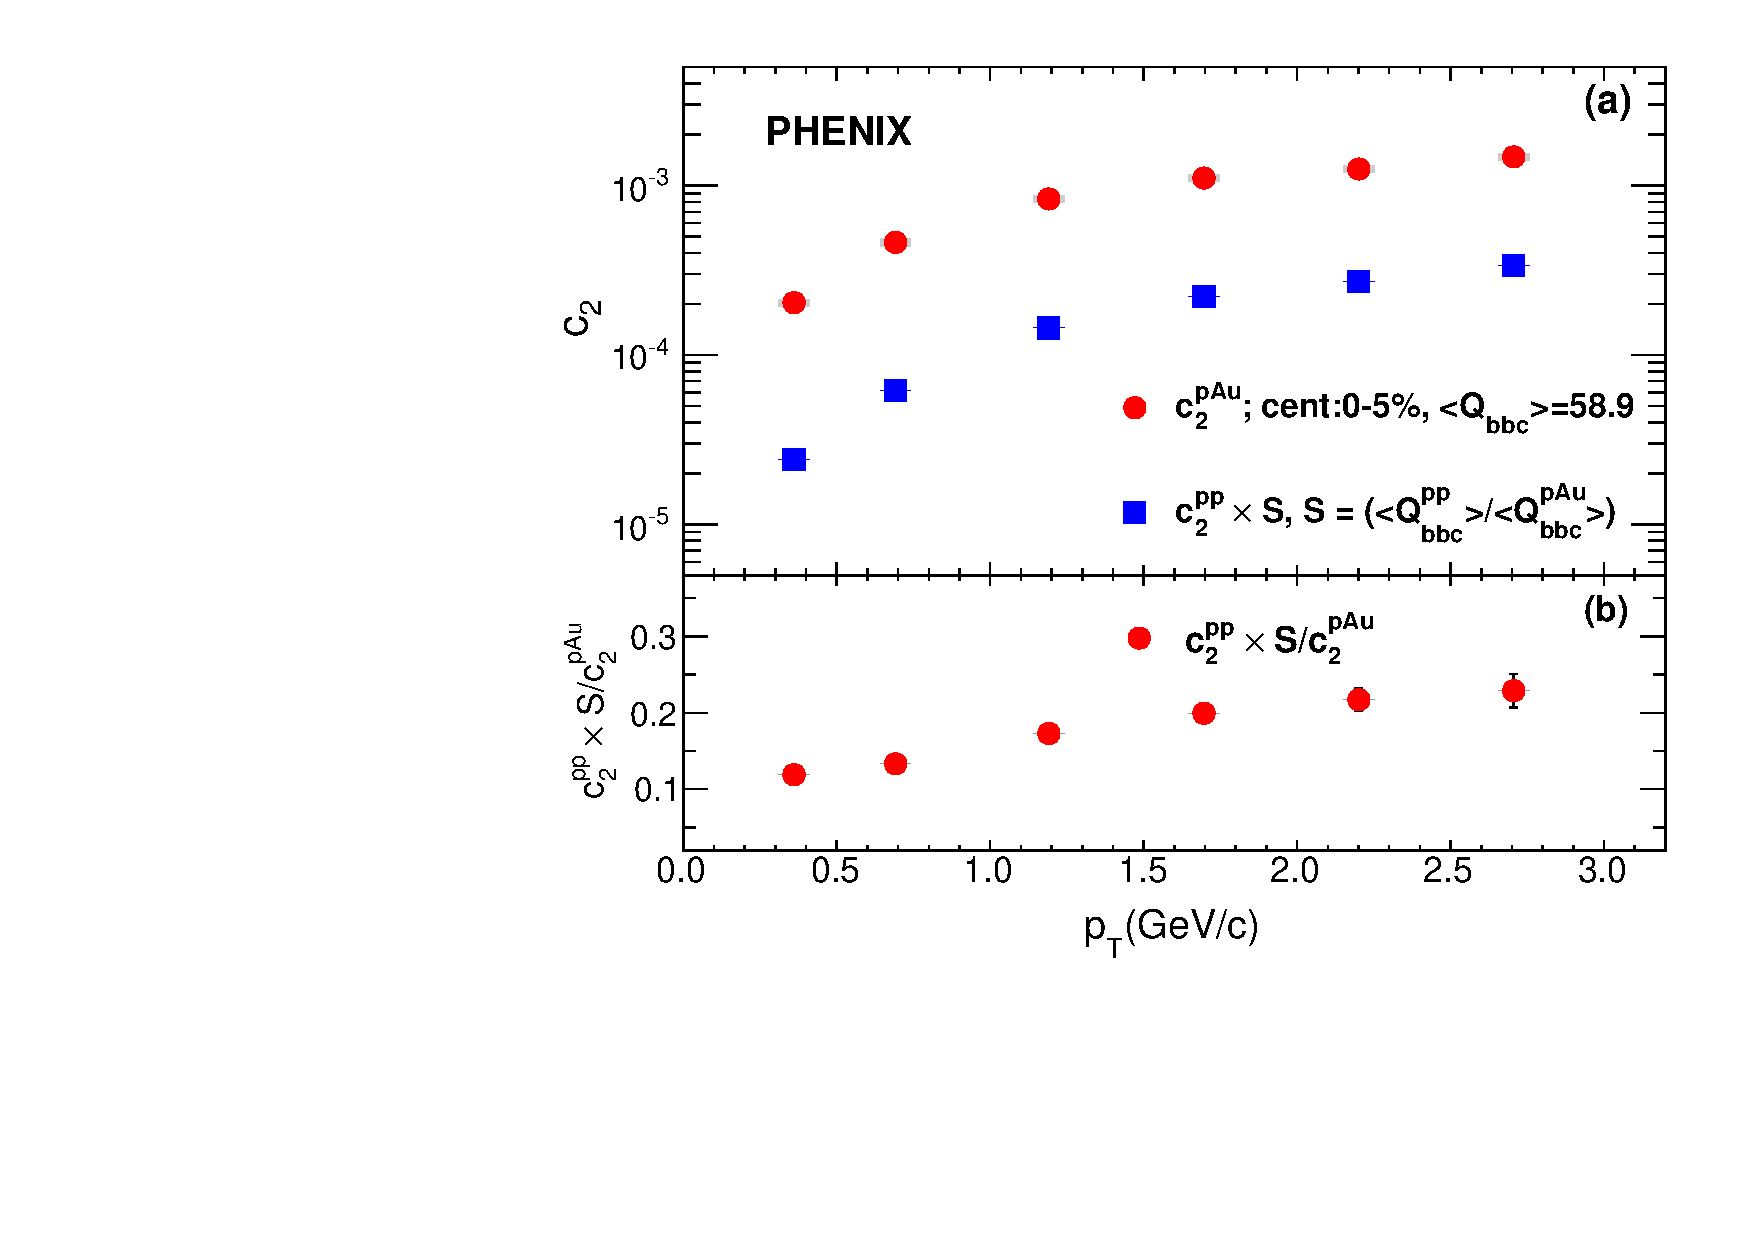
\includegraphics[width=0.6\linewidth]{figs/non_flow.pdf}
\caption{(a) The second order harmonic coefficients $c_2(p_T)$ for long range angular correlations in
0\%--5\% \pau collisions, as well as for minimum bias \pp collisions. The latter are scaled down by the factor $\left( \sum Q^{{\rm \text{BBC-S}}} \right)_{\pp} / \left( \sum Q^{{\rm
\text{BBC-S}}} \right)_{{\rm pAu}}$. (b)~The
ratio of the two harmonics is plotted with the corresponding statistical errors.}
\label{fig:non_flow}
\end{center}
\end{figure}

\section{Systematic Uncertainties Summary}
Table \ref{tbl:sys_uncert} summarizes the sources of systematic uncertainty for the $v_2$ measurement. Each of these systematic uncertainties are categorized by type:
\begin{enumerate}
\item point-to-point uncorrelated between $p_T$ bins,
\item point-to-point correlated between $p_T$ bins,
\item overall normalization uncertainty in which all points are scaled by the same multiplicative factor.
\end{enumerate}
We total the five sources of systematic uncertainty, by adding them in quadrature. The total systematic uncertainty varies from $^{+7.2}_{-13.4}\%$ at low \pt to $^{+7.3}_{-23.8}\%$ at high \pt. Now that the systematic uncertainties have been estimated, we show the $v_2$ physics result in the next chapter.

\begin{table}[!h]
  \begin{center}
  \caption{\label{t:sys}Systematic uncertainties given as a percent of the $v_2$ measurement. Note that the non-flow contribution is $p_T$ dependent and the value here quoted corresponds to the highest measured $p_T$.}
    \begin{tabular}{ccc}
      \hline
      \hline
      Source& Systematic Uncertainty & Type \\ \hline
      Track Background &2.0\%& 1\\ 
      Event Pile-up    &$^{+4}_{-0}\%$& 2\\
      Non-Flow    &$^{+0}_{-23}\%$& 2\\
      Beam Angle &5.0\%& 3\\  
      Event Plane Detectors & 3\% & 3\\
    \hline
    \hline
    \end{tabular}
   \end{center}
   \label{tbl:sys_uncert}
 \end{table}

%\begin{figure}
%\begin{center}
%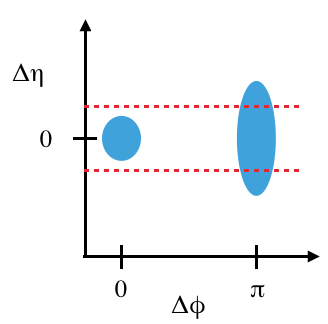
\includegraphics[width=0.5\linewidth]{figs/jet_corr_example.png}
%\caption{TBA}
%\label{fig:jet_corr_example}
%\end{center}
%\end{figure}


%\subsection{Dataset Quality Assurance}
%A PHENIX "run" (lower case r) is defined a group of events that were taken over a single timespan of max length 90 minutes. The for \pau dataset, there are on 
%average 5 million events per run and there are 339 runs. 
%\begin{figure}[!h]
%\begin{center}
%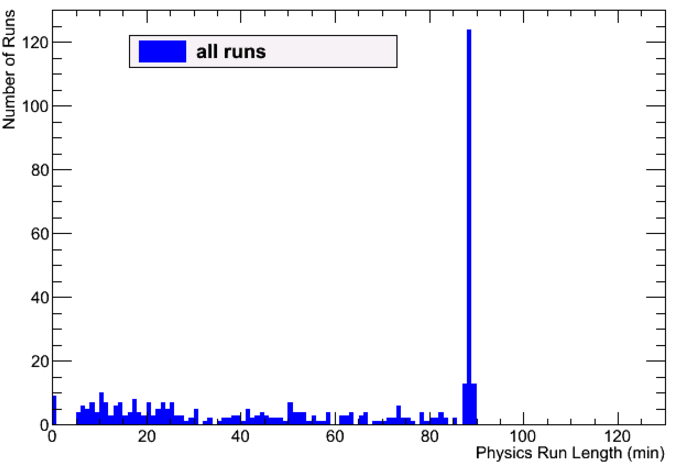
\includegraphics[width=0.65\linewidth]{figs/hruntime.png}
%\caption{The distribution of the length of physics runs.}
%\end{center}
%\end{figure}
%\subsection{luminosity over time}
%RHIC exceeded in delivering its integrated luminosity goals of (\textbf{TO DO: Quantify}).
%\begin{figure}[!h]
%\begin{center}
%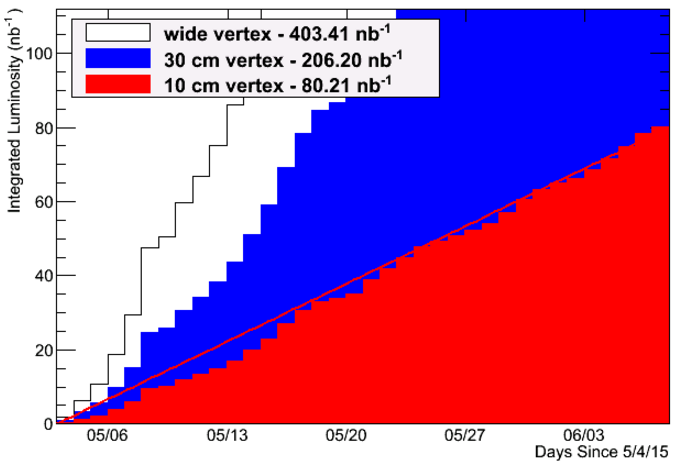
\includegraphics[width=0.65\linewidth]{figs/integrated_luminosity.png}
%\caption{Integrated luminosity from the \pau dataset.}
%\end{center}
%\end{figure}
%\section{bbc charge}
%\begin{figure}[!h]
%\begin{center}
%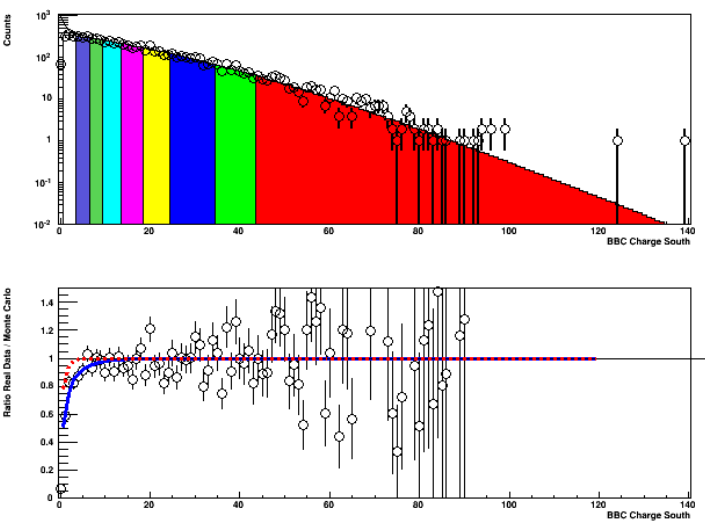
\includegraphics[width=0.65\linewidth]{figs/centrality_determination.png}
%\caption{Real data for BBC Charge South (Au-going direction) shown as open circles and Glauber Monte Carlo + NBD. The colors correspond to the various
%percentiles relative to the total inelastic \pau cross section, the most central 0-5$\%$ in solid red. The blue and red curves correspond to the Leve-1 trigger
%efficiency in all inelastic collisions and inelastic collisions producing a particle at midrapidity, respectively. The best fit NBD parameters are mu = 3.14, k = 0.47
%, and the trigger firing on 84 +/- 3$\%$ of the total inelastic cross section [sigma = 1.76 barns].}
%\end{center}
%\end{figure}
%\begin{figure}[!h]
%\begin{center}
%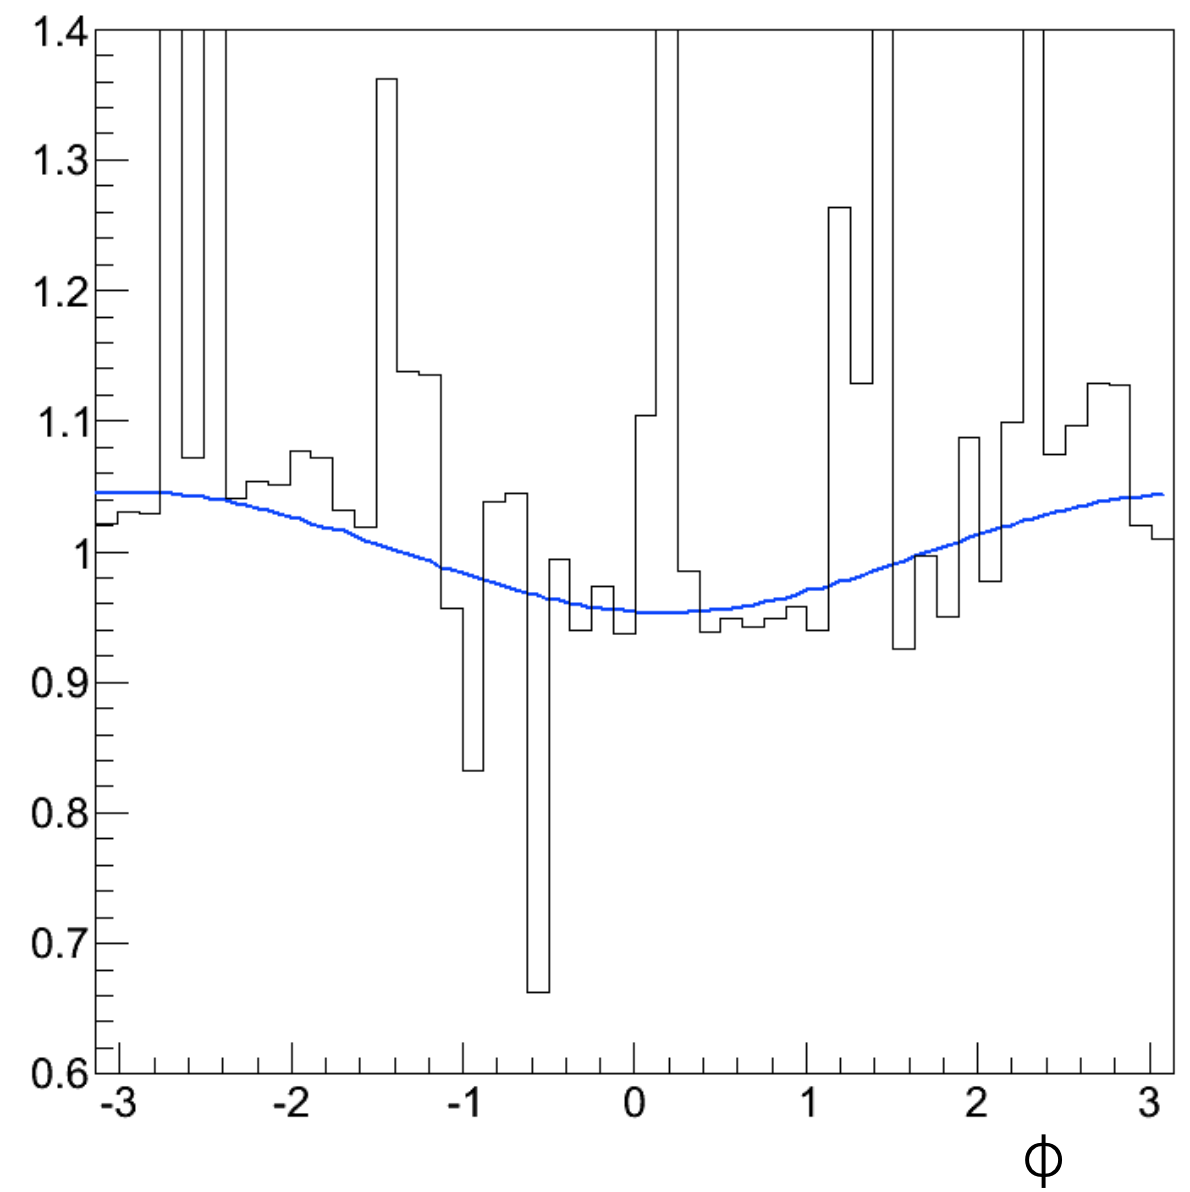
\includegraphics[width=0.5\linewidth]{figs/comparison_of_weights.png}
%\caption{TBA}
%\end{center}
%\end{figure}
%\begin{figure}[!h]
%\begin{center}
%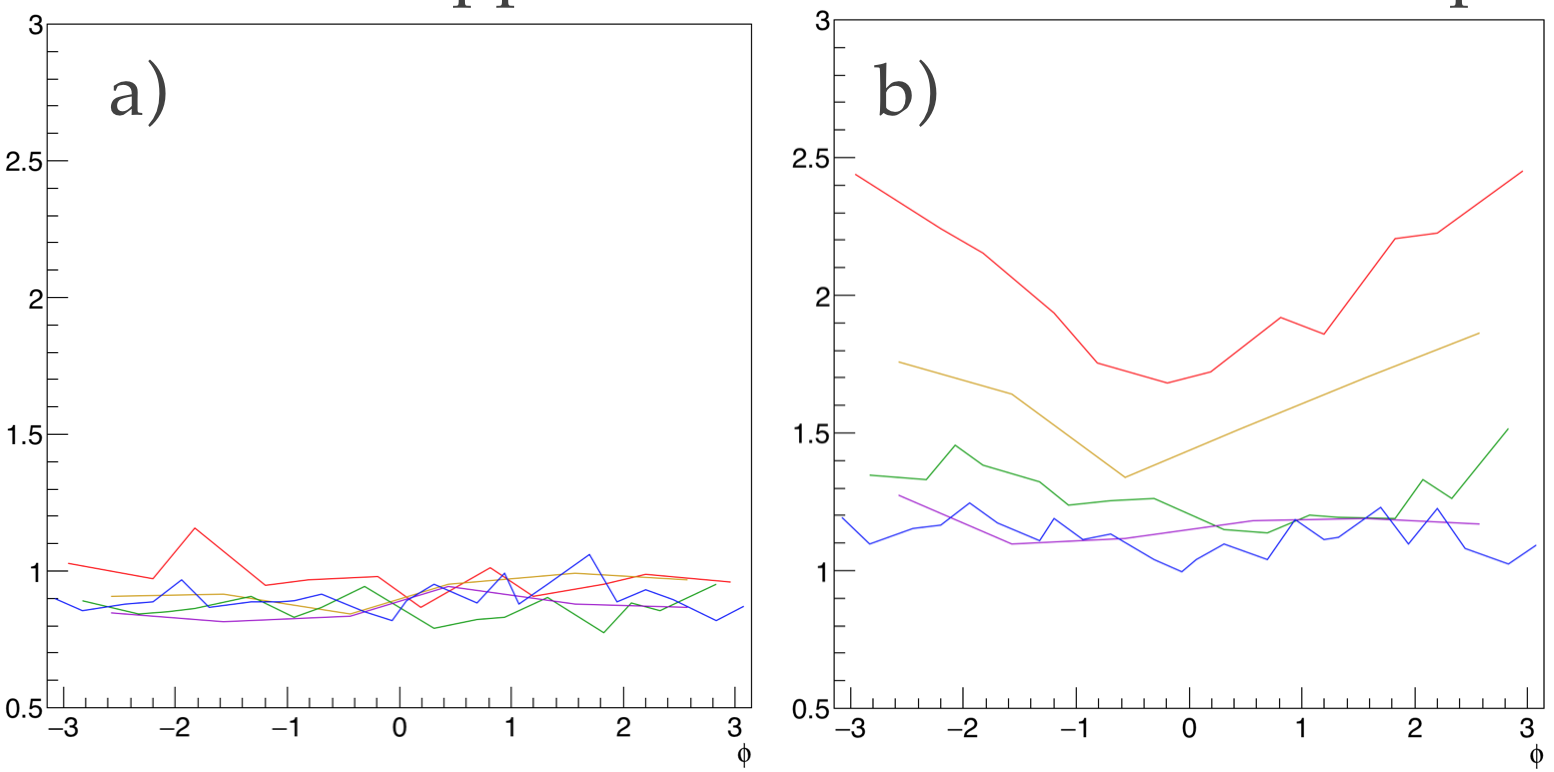
\includegraphics[width=0.6\linewidth]{figs/pp_pau_bbc_comparison.png}
%\caption{These figures show the phi distribution of BBC PMT charge in a) the Run15 pp dataset and in b) the Run15 pAu dataset.}
%\end{center}
%\end{figure}
%\begin{figure}[!h]
%\begin{center}
%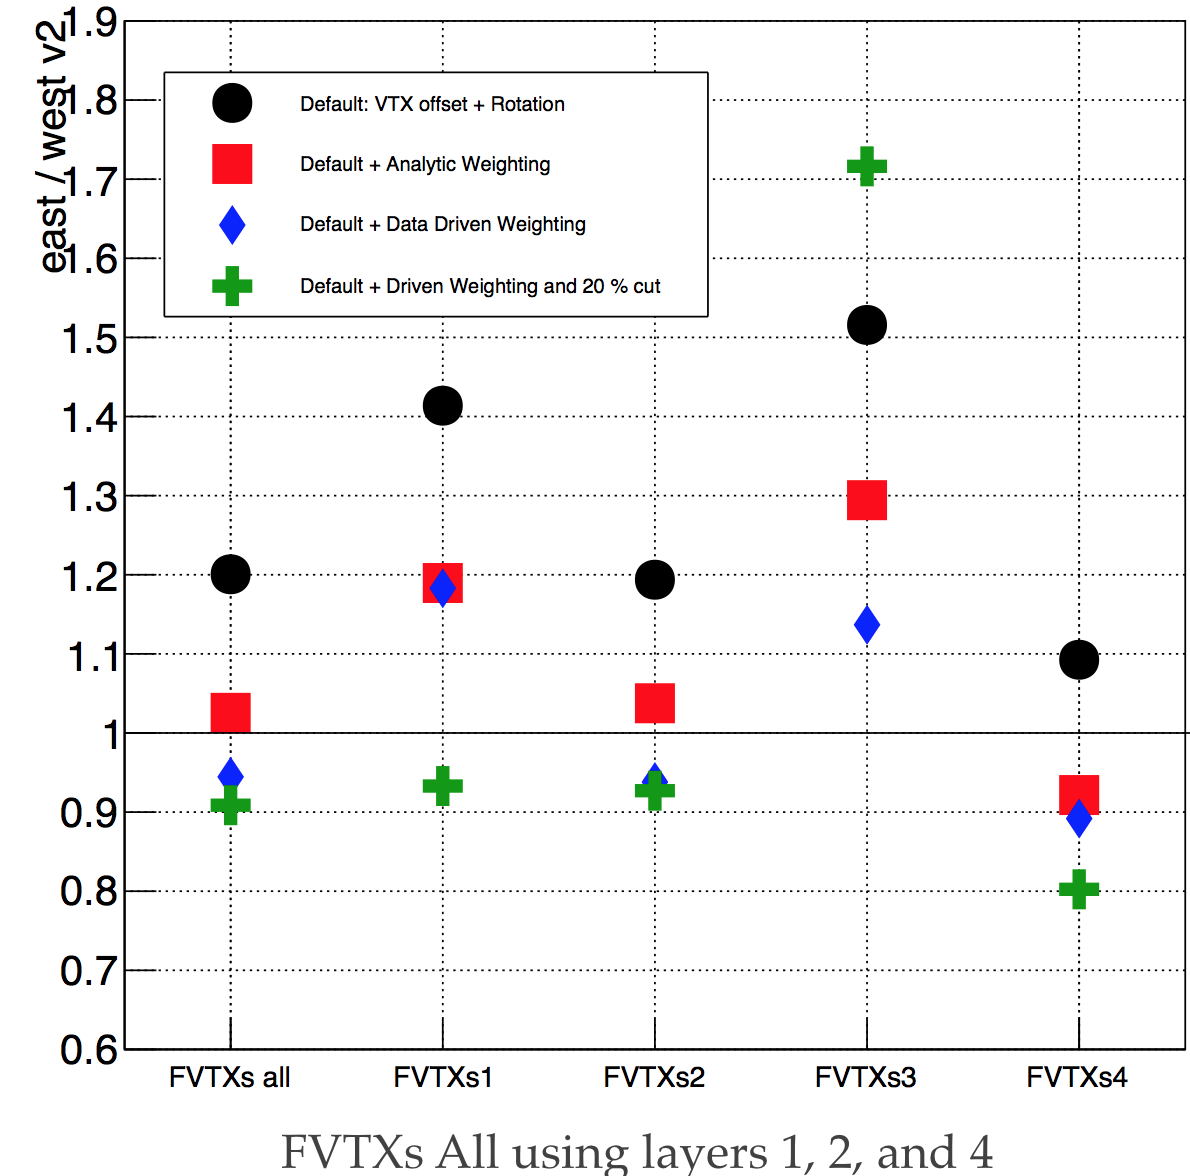
\includegraphics[width=0.5\linewidth]{figs/fvtx_correction_summary.png}
%\caption{TBA}
%\end{center}
%\end{figure}
%\begin{figure}[!h]
%\begin{center}
%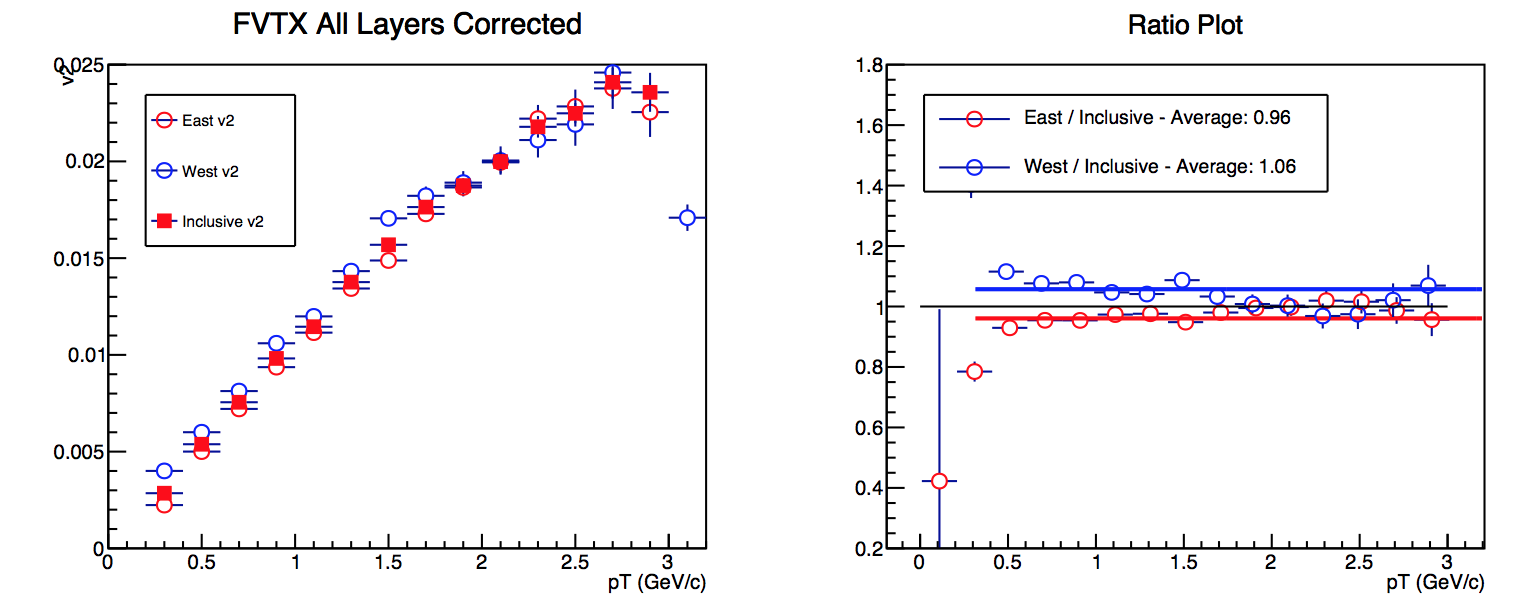
\includegraphics[width=0.5\linewidth]{figs/fvtx_corrected.png}
%\caption{FVTX EP corrected with inverse $\phi$ weighting and 20 $\%$ cut.}
%\end{center}
%\end{figure}
%\begin{figure}[!h]
%\begin{center}
%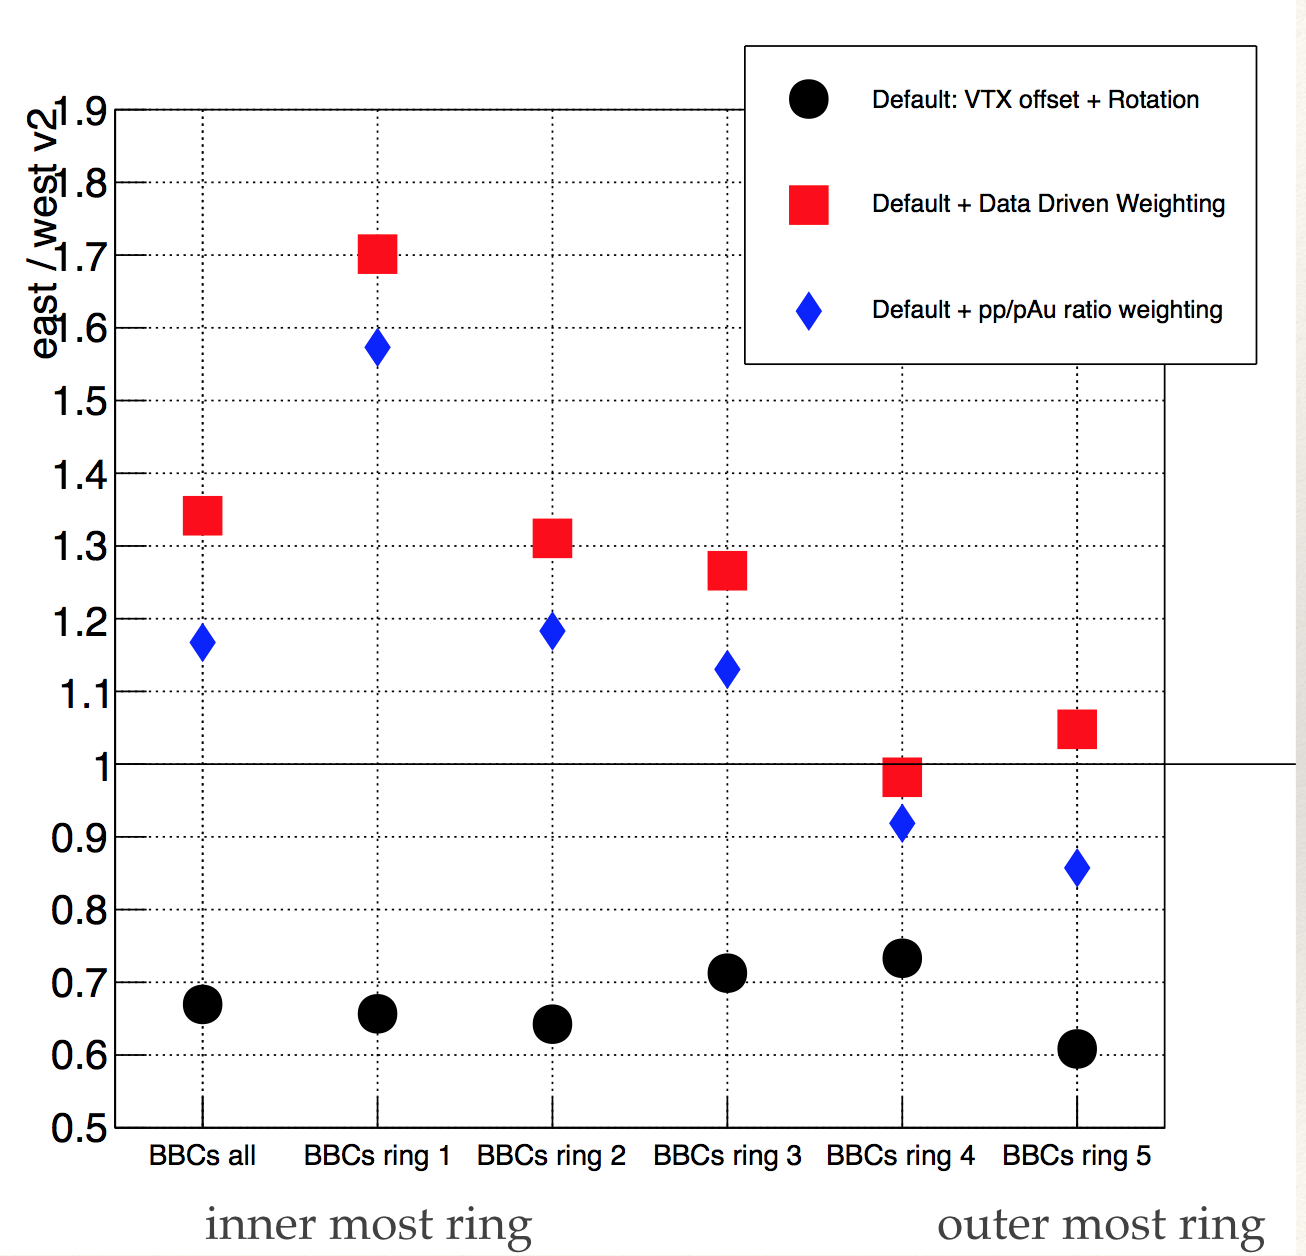
\includegraphics[width=0.5\linewidth]{figs/bbc_correction_summary.png}
%\caption{TBA}
%\end{center}
%\end{figure}
%\begin{figure}[!h]
%\begin{center}
%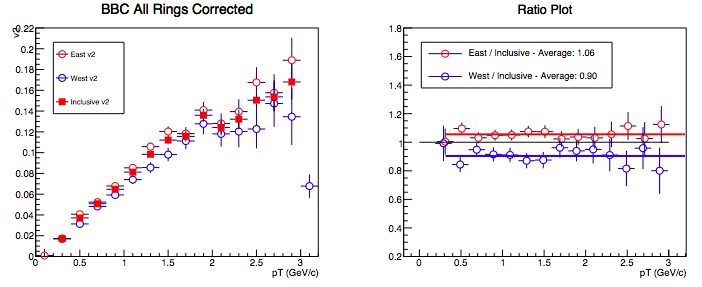
\includegraphics[width=0.5\linewidth]{figs/bbc_pp_correction.png}
%\caption{BBC EP corrected with pp, pau ratio weighting.}
%\end{center}
%\end{figure}
%\begin{figure}[!h]
%\begin{center}
%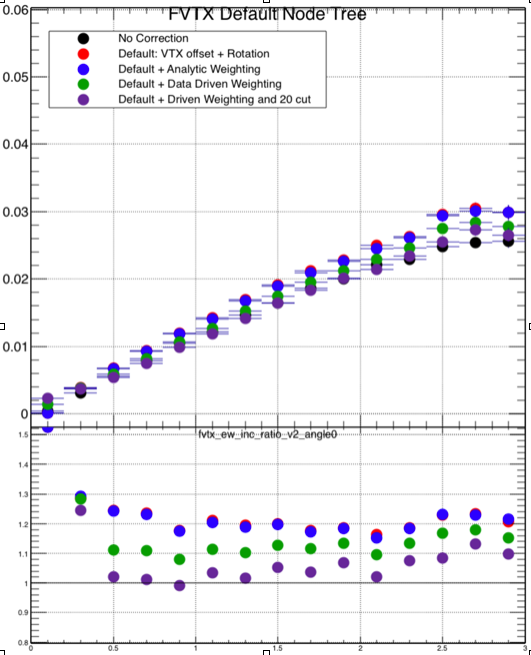
\includegraphics[width=0.5\linewidth]{figs/fvtx_incl_v2_comparison_corrections.png}
%\caption{A comparison of FVTX EP $v_2$ corrections on the inclusive measurement.}
%\end{center}
%\end{figure}
%\section{Systematic Error Estimate}
%\subsection{Non-flow Estimate}
%\begin{figure}[!h]
%\begin{center}
%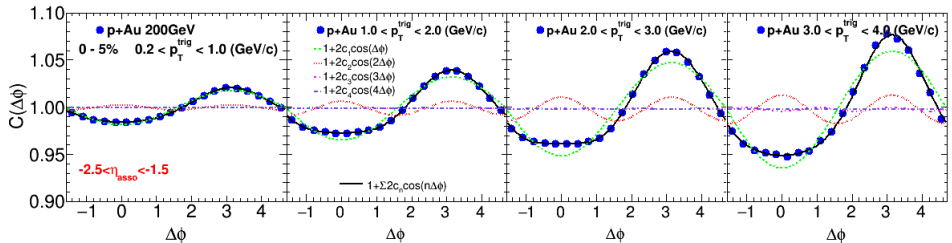
\includegraphics[width=0.6\linewidth]{figs/pau_correlation_central_fvtx.png}
%\caption{TBA}
%\end{center}
%\end{figure}
%\begin{figure}[!h]
%\begin{center}
%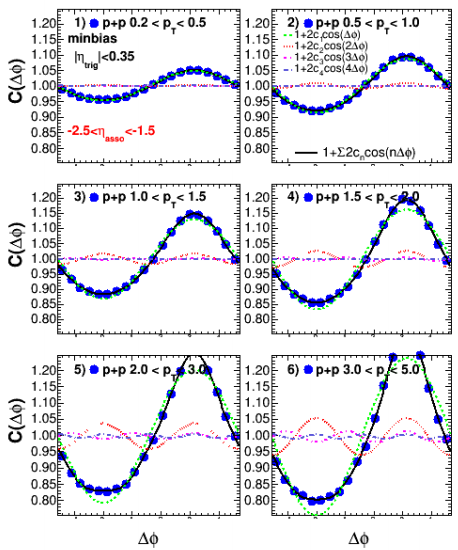
\includegraphics[width=0.6\linewidth]{figs/pp_correlation_minbias_fvtx.png}
%\caption{TBA}
%\end{center}
%\end{figure}
%\begin{figure}[!h]
%\begin{center}
%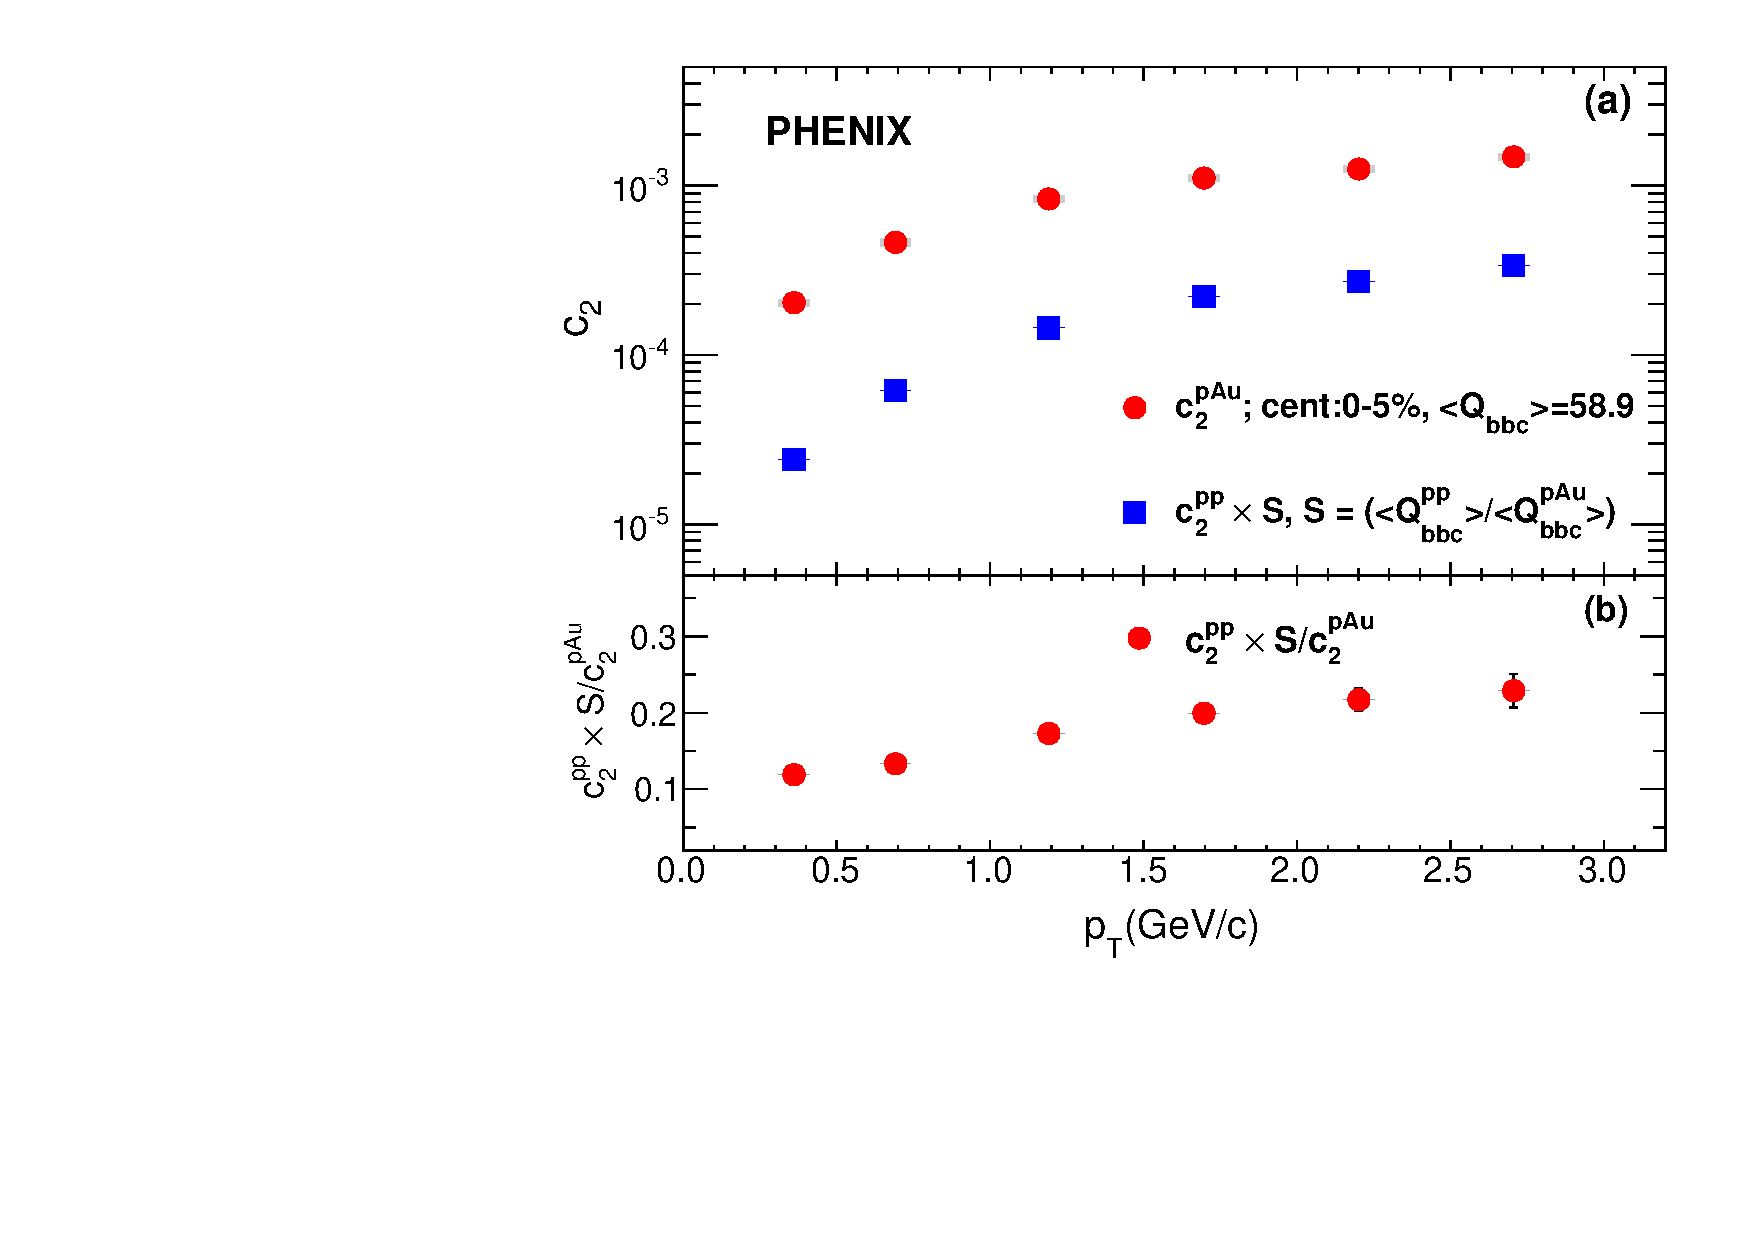
\includegraphics[width=0.6\linewidth]{figs/non_flow.pdf}
%\caption{TBA}
%\end{center}
%\end{figure}
%\subsection{Pile Up}
%\begin{figure}[!h]
%\begin{center}
%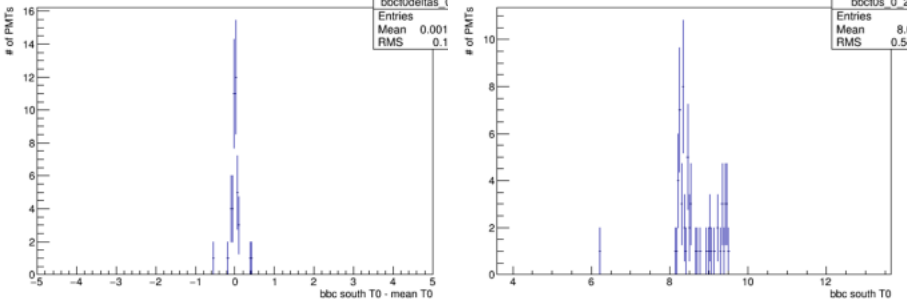
\includegraphics[width=0.6\linewidth]{figs/example_pile_up_event.png}
%\caption{The left plot is an example of a normal event, the right plot is an example pile up event.}
%\end{center}
%\end{figure}
%\subsection{Beam Angle}
%\subsection{Track Background}
%\subsection{Event Plane Detectors Agreement}
